
\chapter{Projeto Conceitual do Produto}

\section{Características gerais}

O produto proposto é um robô autônomo de pequeno porte, denominado Micromouse, cujo objetivo
principal é explorar e resolver labirintos desconhecidos de forma completamente autônoma, sem
qualquer intervenção humana durante o percurso. O robô deverá ser capaz de mapear o ambiente,
monitorar sua própria localização, detectar paredes com $5{,}0\,\text{cm}$ de altura e
$1{,}2\,\text{cm}$ de espessura, e identificar quando alcançou a região central do labirinto,
que corresponde a uma sala retangular de aproximadamente $2 \times 2$ células.

O Micromouse será construído dentro das dimensões máximas de
$25{,}0\,\text{cm} \times 25{,}0\,\text{cm}$, sobre um \textit{chassis} com tração diferencial
de duas rodas motorizadas e uma roda de apoio livre. A navegação será realizada por meio de
três sensores de distância por tempo de voo (\textit{Time of Flight}) VL53L0X, posicionados
nas direções frontal e laterais, complementados por uma unidade de medição inercial MPU6050
responsável pela correção de trajetória nas curvas. O controle dos motores N20 será feito por
uma ponte H TB6612FNG, além disso, eles já apresentam encoder acoplados a cada motor.

O sistema embarcado será gerenciado por um microcontrolador ESP32 DevKitV1, responsável pela
execução do algoritmo de navegação, pelo mapeamento do labirinto em memória e pela comunicação
sem fio via Wi-Fi com a interface de telemetria. O produto contará com monitoramento em tempo
real de tensão e corrente por meio do módulo INA219, exibindo na tela de acompanhamento o tipo
do labirinto, o trajeto percorrido, a velocidade média, o consumo de bateria e o tempo de
conclusão. A alimentação será fornecida por duas células de lítio Lishen LR2170SA em
configuração $2S$, gerenciadas por um BMS 2S 20A com indicador de carga, e reguladas por um
conversor Buck DC-DC para $5{,}0\,\text{V}$.

Para garantir a viabilidade e a qualidade das entregas, foi elaborada uma Estrutura Analítica
do Projeto (EAP), que pode ser visualizada na Figura~\ref{fig:eap}.

\begin{landscape}
    \begin{figure}[htbp]
        \centering
        \includesvg[width=1\linewidth]{figuras/EAP}
        \caption{Estrutura Analítica do Projeto}
        \label{fig:eap}
    \end{figure}
\end{landscape}

\section{Estrutura}

\subsection{Introdução}
Esta seção reúne as análises e decisões referentes ao planejamento estrutural e mecânico do Micromouse. Inclui o desenho do chassi, a definição dos materiais, a organização interna do esqueleto e a escolha do sistema de locomoção, seja bimotor ou com soluções de tração mais complexas. Abrange também a especificação dos motores que garantirão mobilidade adequada e a análise de componentes adicionais, como ventoinhas voltadas à estabilidade.

Além disso, contempla a metodologia utilizada para o desenvolvimento do labirinto de testes, seguindo rigorosamente o padrão oficial de dimensões e acabamento, permitindo a validação realista do desempenho do robô.

\subsection{Modelos CAD da Estrutura}
Abaixo, estão apresentadas, em CAD e desenvolvidas no SolidWorks, as imagens do chassi do micromouse, de sua montagem com os componentes, além dos pinos, paredes e piso do labirinto de testes. As paredes, os pinos e o chassi serão fabricados por impressão 3D, enquanto o piso do labirinto será confeccionado em MDF.

Os modelos CAD podem ser observados na Figura~\ref{fig:CADs}

\begin{figure}[H]
    \centering
    
    \begin{subfigure}[b]{0.40\textwidth}
        \centering
        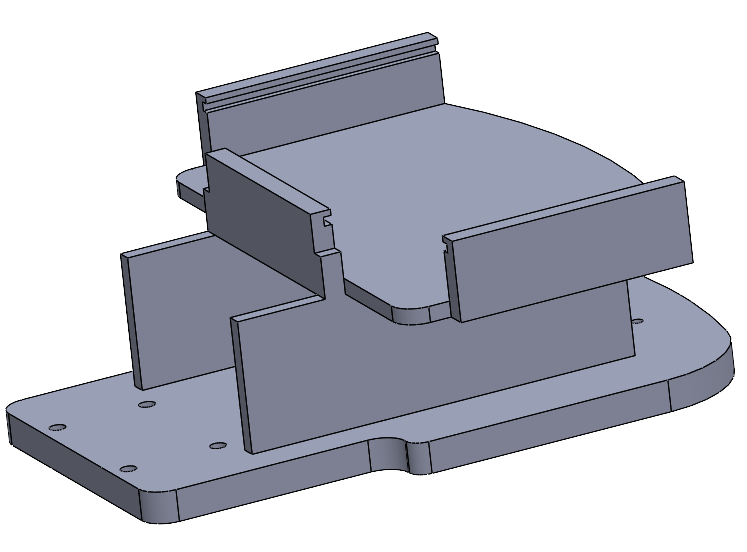
\includegraphics[width=\textwidth]{figuras/Chassi.png}
        \caption{Chassi do micromouse}
        \label{fig:CadChassi}
    \end{subfigure}
    \hfill 
    \begin{subfigure}[b]{0.40\textwidth}
        \centering
        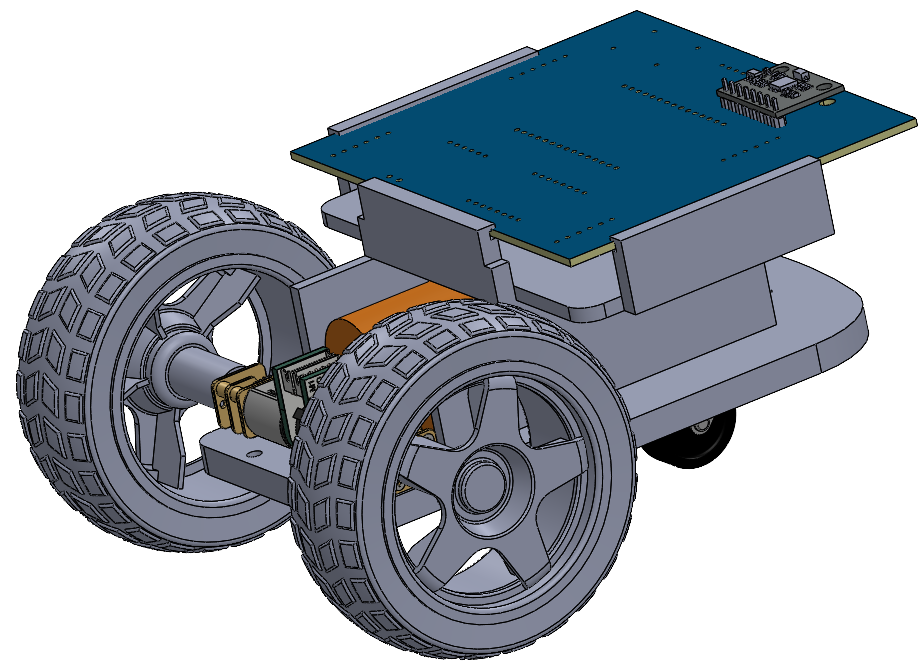
\includegraphics[width=\textwidth]{figuras/Assembly_MrBombastic.png}
        \caption{Assembly do micromouse}
        \label{fig:AssemblyMrBombastic}
    \end{subfigure}
    
    \begin{subfigure}[b]{0.40\textwidth}
        \centering
        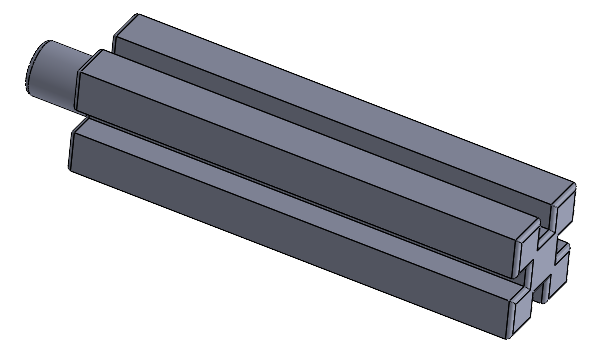
\includegraphics[width=\textwidth]{figuras/Pino_de_fixação_das_paredes.png}
        \caption{Pinos de fixação das paredes}
        \label{fig:CadPinos}
    \end{subfigure}
    \hfill
    \begin{subfigure}[b]{0.40\textwidth}
        \centering
        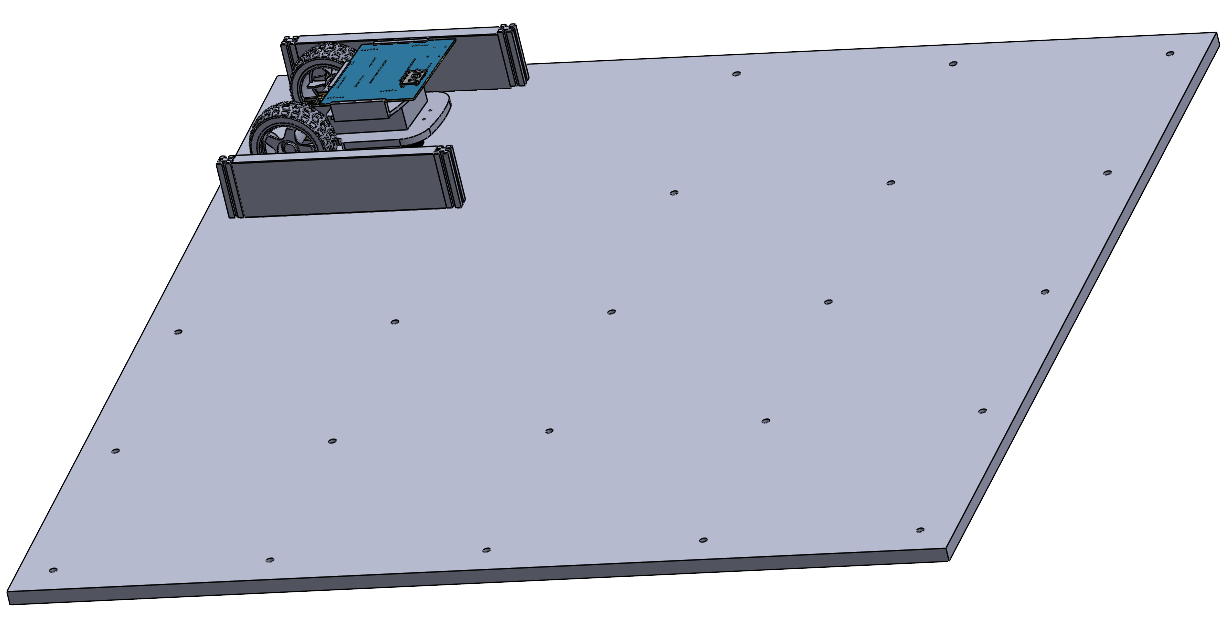
\includegraphics[width=\textwidth]{figuras/Labirinto_de_testes_Assembly.png}
        \caption{Montagem do labirinto}
        \label{fig:AssemblyLabirinto}
    \end{subfigure}
    
    \caption{CADs do projeto}
    \label{fig:CADs}
\end{figure}

Na tabela a seguir, estão descritas as dimensões dos desenhos em CAD, com suas respectivas alturas, comprimentos e larguras.

\begin{table}[H]
    \centering
    \caption{Dimensões das peças}
    \label{tab:dimensoes_pecas}
    \begin{tabular}{|c|c|c|c|}
        \hline
        \textbf{Item} & \textbf{Comprimento [mm]} & \textbf{Altura [mm]} & \textbf{Largura [mm]} \\ \hline
        (a) &120,21 &46,35 &105 \\ \hline
        (b) &146,93 &68,55 &121,92 \\ \hline
        (c) &12 &12 &57 \\ \hline
        (d) &780 &12 &780 \\ \hline
    \end{tabular}
\end{table}

\subsection{Decisões do projeto}

\subsubsection{Planejamento do Chassi}
O chassi do micromouse será desenvolvido baseado ao Projeto Jabuti \cite{Projeto_Jabuti} com o uso da impressora 3D, usando como material, o \textbf{filamento PLA} para sua construção. No projeto do chassi, a bateria foi posicionada próxima ao centroide da estrutura por ser o componente de maior massa do sistema. Essa configuração contribui para uma melhor distribuição de peso, garantindo maior estabilidade durante o movimento e reduzindo a necessidade de adicionar massas extras para balanceamento do micromouse. Além disso, o posicionamento central auxilia na diminuição da tendência de inclinação durante curvas, melhorando o desempenho dinâmico do micromouse.

\subsubsubsection{Justificativa para a escolha da \textbf{impressora 3D}}
As principais vantagens de usar a impressora 3D para a construção do chassi do micromouse são:

\begin{enumerate}
    \item \textbf{Liberdade Absoluta para Posicionamento de Sensores:} Trazendo a possibilidade de desenhar suportes inclinados e embutidos para os sensores de distância.
    
    \item \textbf{Prototipagem Rápida e Design Iterativo:} A impressão 3D permite ajustar o CAD e fabricar uma nova base em poucas horas, acelerando o ciclo de desenvolvimento.
    
    \item \textbf{Otimização de Peso e Customização Estrutural:} A impressão 3D permite controlar a densidade interna da peça. Ajustando o preenchimento. Logo, o chassi torna-se extremamente leve, permitindo reforços estruturais apenas nos pontos de maior estresse físico.

    \item \textbf{Facilidade:} Tendo em vista que um dos integrantes possui a impressora 3D, torna mais fácil fazer as alterações necessárias do chassi do micromouse.
\end{enumerate}

\subsubsection{Sistema de Locomoção}
Para o sistema de locomoção será utilizado 3 rodas, uma ao centro do micromouse para sustentação e as outras duas para movimentação e curvas nas laterais traseiras do carrinho. A escolha do conjunto de rodas baseou-se em critérios de confiabilidade técnica, integração estrutural e eficiência em simetria com a pista de testes. As especificações das rodas são as seguintes:

\begin{table}[htbp]
    \centering
    \caption{Rodas de movimentação}
    \label{tab:placeholder}
    \begin{tabular}{|c|c|} \hline
        Diâmetro & 68mm \\ \hline
        Largura & 26mm \\ \hline
        Furo central & 5,3mm x 3,66mm (Semicírculo) \\ \hline
        Peso & 50g \\ \hline
    \end{tabular}
\end{table}

\begin{table}[htbp]
    \centering
    \caption{Roda de sustentação}
    \label{tab:placeholder}
    \begin{tabular}{|c|c|} \hline
        Diâmetro & 19mm \\ \hline
        Largura & 7,9mm \\ \hline
        Furo central & $\varnothing$ 2,36mm \\ \hline
    \end{tabular}
\end{table}

\subsubsection{Labirinto de Testes}
A construção do labirinto de testes foi baseada na estrutura feita pela UKMARS (Sociedade Britânica de Micromouse e Robótica) \cite{ukmars_maze}. Para o piso, será utilizado o material \textbf{MDF (\textit{Medium-Density Fiberboard})}, enquanto as paredes e pinos de sustentação serão confeccionados em \textbf{impressora 3D}. O labirinto de testes foi desenvolvido de forma que permitisse a alteração da posição das paredes, possibilitando diferentes configurações de percurso. Dessa maneira, torna-se possível realizar testes em variados cenários, ampliando as possibilidades de validação do funcionamento do micromouse e permitindo a análise de seu desempenho em trajetórias com diferentes níveis de complexidade.

\subsubsubsection{Justificativa da Escolha do MDF para o piso}
As principais vantagens de utilizar o \textbf{MDF} são: 

\begin{enumerate}
    \item \textbf{Superfície Lisa e Sem Veios:} Ao contrário da madeira compensada ou maciça, o MDF não possui ``veios'', nós ou irregularidades naturais. Isso é fundamental para a Odometria Precisa e a Leitura de Sensores do Micromouse.
    
    \item \textbf{Excelente Acabamento para Pintura:} O piso do labirinto de Micromouse precisa ser pintado de preto para criar alto contraste. O MDF absorve muito bem as tintas, permitindo um acabamento liso e sem reflexos, o que é crucial para que a luz ambiente ou os emissores do robô não causem leituras erradas nos sensores de parede.
    
    \item \textbf{Alta Precisão de Corte e Usinagem:} Devido as células do labirinto terem um padrão de medidas muito rígidas ($18\,\text{cm} \times 18\,\text{cm}$). O MDF é extremamente fácil de cortar com serras circulares ou máquinas de corte a laser/CNC sem lascar as bordas. 
    
    \item \textbf{Estabilidade Dimensional (em ambientes internos):} Desde que mantido longe de umidade, o MDF é muito mais estável que a madeira comum. Ele não empena ou torce facilmente com variações normais de temperatura, garantindo que o seu piso fique perfeitamente nivelado. Um piso desnivelado pode fazer o robô raspar o chassi ou perder a calibração do giroscópio.
    
    \item \textbf{Custo-Benefício:} Construir o piso com materiais como acrílico fosco, polímeros de engenharia ou metais seria financeiramente inviável para o projeto. O MDF oferece um equilíbrio perfeito entre qualidade profissional e preço acessível.    
\end{enumerate}

\subsubsubsection{Justificativa da Escolha da impressora 3D}
As principais vantagens de utilizar a \textbf{Impressora 3D} são:

\begin{enumerate}
    \item \textbf{Cores Nativas:} Com a impressora 3D, pode-se simplesmente usar filamento branco para a parede e usar filamento vermelho para o topo. Isso economiza horas de isolamento com fita crepe, aplicação de primer e secagem de tinta, além de evitar o risco da tinta descascar com as batidas do robô.
    
    \item \textbf{Design de Encaixe Perfeito (Tolerâncias Customizadas):} É possível modelar os pinos com tolerâncias exatas para o diâmetro dos furos que serão feitos no MDF e para a espessura das paredes.
    
    \item \textbf{Reprodutibilidade e Precisão Dimensional:} O labirinto exige dezenas de paredes e pinos idênticos. A impressora 3D garante que a parede número 1 terá exatamente as mesmas dimensões da parede número 80. Diferente de cortar madeira ou acrílico manualmente, onde erros milimétricos se acumulam e estragam o \textit{grid} da pista, a impressora entrega consistência.
    
    \item \textbf{Baixo Peso com Boa Resistência:} Filamentos comuns como PLA ou PETG são mais do que resistentes o suficiente para aguentar os impactos de um Micromouse.
    
    \item \textbf{Facilidade:} Tendo em vista que um dos integrantes possui a impressora 3D, torna mais fácil fazer as alterações necessárias e ajustes das paredes e pinos do labirinto.
\end{enumerate}

% ============================================================
% SEÇÃO 4.3 — DESCRIÇÃO DE HARDWARE (ATUALIZADA)
% ============================================================
\section{Descrição de \textit{hardware}}

O \textit{hardware} proposto para o sistema foi projetado a partir de uma arquitetura modular
para um robô móvel autônomo, com foco em processamento eficiente, sensoriamento preciso e
monitoramento energético. A arquitetura é organizada em quatro módulos principais:
\textbf{Processamento}, \textbf{Sensoriamento}, \textbf{Atuação} e \textbf{Gerenciamento de
Energia}. A organização sistêmica entre esses módulos pode ser visualizada no diagrama de
blocos da Figura~\ref{fig:diag.blocos}, enquanto as conexões elétricas detalhadas entre os
componentes são apresentadas nos esquemáticos das Figuras~\ref{fig:esque.princi}
e~\ref{fig:esque.bms}.

Toda a eletrônica do sistema será montada sobre \textbf{placa perfurada} (\textit{perfboard}),
permitindo a integração compacta dos componentes de forma modular, reutilizável e de custo
reduzido, sem a necessidade de fabricação de uma \textit{Printed Circuit Board} (PCB) dedicada
nesta fase do projeto.

\begin{figure}[H]
    \centering
    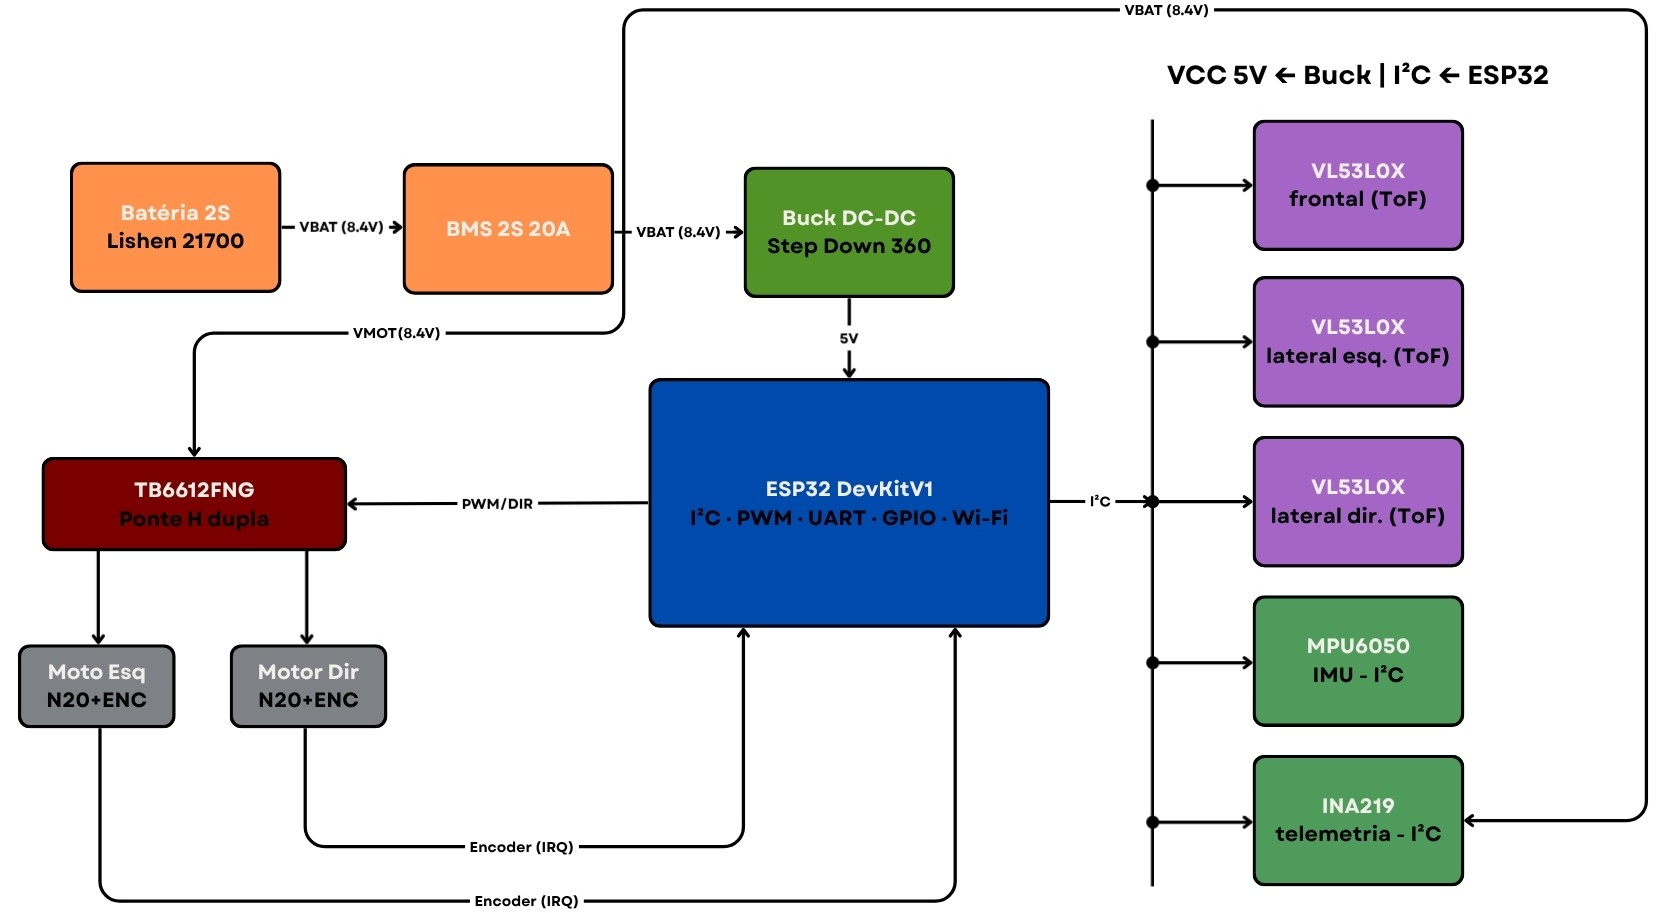
\includegraphics[width=0.75\linewidth]{figuras/Diagrama de Blocos (Hardware) - PI1.jpg}
    \caption{Diagrama de Blocos}
    \label{fig:diag.blocos}
\end{figure}

\begin{figure}[H]
    \centering
    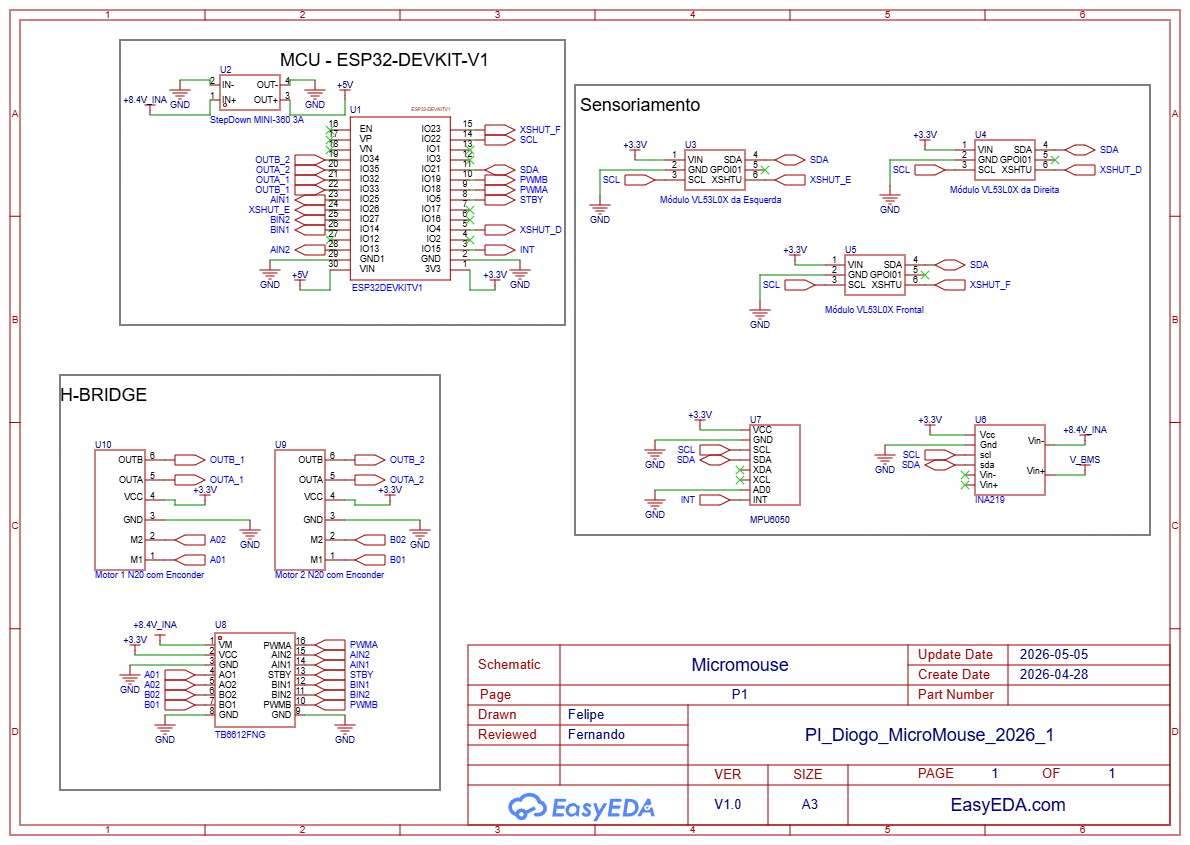
\includegraphics[width=0.8\linewidth]{figuras/Esquemático_principal.png}
    \caption{Esquemático Principal do Hardware}
    \label{fig:esque.princi}
\end{figure}

\begin{figure}[H]
    \centering
    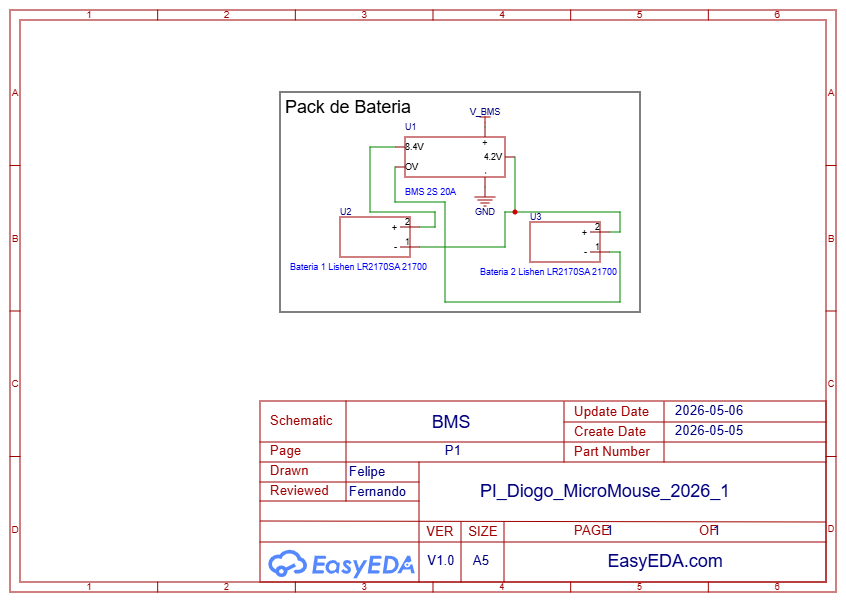
\includegraphics[width=0.8\linewidth]{figuras/Esquemático_BMS.png}
    \caption{Esquemático do pack de baterias}
    \label{fig:esque.bms}
\end{figure}

\subsection{Módulo de Processamento}

O núcleo do sistema é o microcontrolador \textbf{ESP32 DevKitV1}, baseado no SoC ESP32 da
Espressif Systems. Sua escolha se justifica pela necessidade de processar dados provenientes
de múltiplos sensores no barramento $I^2C$ em tempo real, executar o algoritmo de navegação e
mapeamento do labirinto em memória, além de realizar comunicação sem fio via \textit{Wi-Fi}
para telemetria. O ESP32 opera com clock de até 240\,MHz com dois núcleos, possui 520\,KB de
RAM e 4\,MB de Flash, e suporta nativamente os protocolos $I^2C$, UART, SPI e PWM, todos
utilizados neste projeto. A programação é realizada via USB utilizando a Arduino IDE com o
\textit{core} ESP32 da Espressif.

\subsection{Módulo de Sensoriamento}

\subsubsection{Sensores de Distância VL53L0X}

O sensor \textbf{VL53L0X} é um módulo de distância por \textit{Time of Flight} (ToF) fabricado
pela STMicroelectronics. Diferentemente de sensores infravermelhos analógicos, o VL53L0X emite
pulsos de luz laser infravermelha (850\,nm) e mede o tempo de retorno para calcular a distância
com precisão de até 1\,mm e alcance de até 2\,m em condições ideais. No contexto do Micromouse,
onde as paredes do labirinto distam entre 0 e 18\,cm, este sensor oferece excelente resolução
e imunidade a variações de cor e refletividade da superfície.

Serão utilizados três módulos VL53L0X: um posicionado na frente do robô (Frontal) e
dois nas laterais (Esquerda e Direita), possibilitando a detecção de paredes em todas as
direções relevantes à navegação. Todos os sensores compartilham o barramento $I^2C$ com o
ESP32. Para que dispositivos com o mesmo endereço padrão possam coexistir no barramento, cada
sensor possui um pino \texttt{XSHUT} conectado a uma GPIO do ESP32, permitindo que cada
unidade seja inicializada individualmente e tenha seu endereço $I^2C$ reconfigurado por
software antes de ser liberada para operação.

\subsubsection{Unidade de Medição Inercial MPU6050}

O \textbf{MPU6050} é uma IMU (\textit{Inertial Measurement Unit}) de 6 eixos, combinando
acelerômetro e giroscópio em um único encapsulamento com interface $I^2C$. No sistema, ele é
responsável pela estimativa da orientação angular (\textit{heading}) do robô durante as curvas,
complementando os dados dos sensores ToF e dos encoders. O giroscópio fornece a taxa de rotação
em torno do eixo Z (yaw), permitindo ao algoritmo de controle corrigir desvios angulares e
garantir que as curvas de 90° sejam executadas com precisão.

\subsubsection{Sensor de Corrente e Tensão INA219}

O \textbf{INA219} é um sensor de corrente e tensão bidirecional da Texas Instruments com
interface $I^2C$. Ele é inserido em série no barramento de alimentação do sistema e realiza a
medição da tensão na carga e da corrente consumida por meio de um resistor \textit{shunt} de
precisão (0,1\,$\Omega$). Com resolução de 12 bits e faixa de medição de até 3,2\,A e 32\,V,
o INA219 permite o monitoramento contínuo do consumo energético em tempo real. Os dados
coletados são utilizados pelo firmware para calcular a potência instantânea, estimar a
autonomia restante da bateria e acionar alertas de subtensão, sendo também transmitidos via
\textit{Wi-Fi} para o painel de telemetria.

\subsubsection{Encoders dos Motores}

Os motores N20 selecionados já possuem encoders magnéticos acoplados ao eixo traseiro.
Cada encoder gera pulsos por interrupção nas GPIOs do ESP32, permitindo o cálculo da velocidade
de rotação (RPM) e do deslocamento linear percorrido por cada roda. Esses dados são fundamentais
para a implementação do controle PID de velocidade e para a odometria, possibilitando que o
robô estime sua posição relativa dentro do labirinto.

\subsection{Módulo de Atuação}

\subsubsection{Motores N20 com Redução}

Os atuadores de locomoção são dois motores \textbf{DC N20} com caixa de redução, escolhidos
pelo seu tamanho compacto, baixo peso e torque adequado para a massa estimada do robô. Cada
motor é controlado individualmente por um canal do driver TB6612FNG, recebendo sinais de
direção e PWM provenientes do ESP32.

\subsubsection{Driver de Motor TB6612FNG}

O \textbf{TB6612FNG} é um driver de ponte H dupla da Toshiba capaz de acionar dois motores DC
de forma independente. Opera com tensão de motor de até 15\,V e corrente contínua de 1,2\,A
por canal, suportando picos de 3,2\,A. O controle de direção é feito pelos pinos
\texttt{AIN1}/\texttt{AIN2} e \texttt{BIN1}/\texttt{BIN2}, enquanto a velocidade é modulada
pelos pinos \texttt{PWMA} e \texttt{PWMB} via sinal PWM gerado pelo ESP32. O pino \texttt{STBY}
deve ser mantido em nível alto para habilitar a operação do \textit{chip}.

\subsection{Módulo de Gerenciamento de Energia}

A alimentação do sistema é fornecida por duas células de lítio-íon \textbf{Lishen LR2170SA
(21700)} em configuração 2S1P, totalizando 4000\,mAh e tensão nominal de 7,4\,V (8,4\,V
carregadas). Um \textbf{BMS 2S 20A} (modelo HW-391) é responsável pela proteção contra
sobrecarga, subdescarga e curto-circuito, além de realizar o balanceamento das células durante
a carga. Para a alimentação da lógica, um conversor \textbf{Buck DC-DC Step Down 360} regula
a tensão de entrada para 5\,V estáveis, que alimentam o ESP32 pelo pino \texttt{VIN}. Os
motores são alimentados diretamente pelo barramento de bateria (7,4\,V -- 8,4\,V). O
esquemático do pack de baterias com a BMS é apresentado na Figura~\ref{fig:esque.bms}.

\begin{comment}
\textcolor{red}{A descrição de \textit{hardware} no documento deve permitir que outras pessoas repliquem o produto proposto neste documento. Para isso, deve-se explicar de forma textual os principais sub-sistemas e as escolhas de projeto, além de indicar:}

\begin{itemize}
    \item \textcolor{red}{ O diagrama de blocos \cite{blockdiagram}, que oferece uma visão geral do hardware, com as principais partes do sistema e as ligações entre elas.}
    %\item A lista de materiais \cite{bom}, que facilita a montagem do sistema, indicando tudo que deve ser adquirido. Aproveitem a lista de materiais para apresentarem o orçamento dos mesmos.
    \item \textcolor{red}{ O esquemático \cite{esquematico}, que mostra as conexões elétricas entre os componentes. Deve-se indicar os componentes por nomes e símbolos, e as conexões entre eles, incluindo a pinagem dos componentes. Se o esquemático ficar muito grande, pode-se separa-lo em vários esquemáticos. A ligação em \textit{protoboard} não é considerada um esquemático adequado.}
\end{itemize}

\textcolor{red}{A Fig. \ref{fig:diagrama_blocos_e_esquematico} apresenta o diagrama de blocos e o esquemático de um circuito conversor de corrente alternada para corrente direta, a título de exemplo. Repare que o diagrama de blocos indica os sub-sistemas do circuito completo apresentado no esquemático. 
% Comecem com o diagrama de blocos, que é mais genérico, e depois indiquem os detalhes com a lista de materiais e os esquemáticos.
}

\begin{figure}
    \centering
    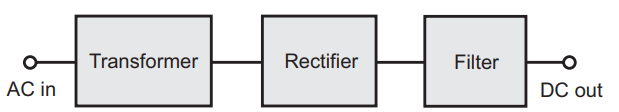
\includegraphics[width=0.5\linewidth]{figuras/Exemplo-diagrama-de-blocos.png}
    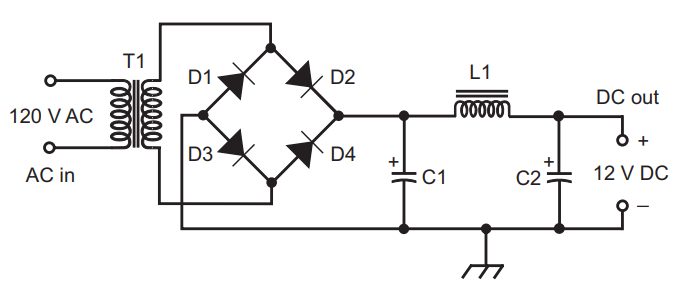
\includegraphics[width=0.5\linewidth]{figuras/Esquematico.png}
    \caption{\textcolor{red}{Diagrama de blocos e esquemático de um circuito conversor de corrente alternada para corrente direta. Extraído de \cite{block_n_schematic}.}}
    \label{fig:diagrama_blocos_e_esquematico}
\end{figure}
\end{comment}

\section{Análise de Consumo Energético}

A análise de consumo energético do micromouse é fundamental para garantir a autonomia necessária durante a execução dos desafios propostos, assegurando estabilidade operacional e prevenindo quedas de tensão que possam comprometer a navegação. Nesta seção, detalham-se os subsistemas elétricos, os cálculos de consumo individual e total, a seleção da fonte de alimentação e os mecanismos de regulação e monitoramento.

\subsection{Identificação dos Subsistemas Elétricos}

Os componentes foram classificados de acordo com sua função no sistema e caracterizados pela tensão de operação, corrente média consumida e tempo aproximado de uso durante um ciclo típico de execução de dez minutos. A configuração final inclui três sensores de distância por tempo de voo (ToF) e uma unidade de medição inercial (IMU) para controle de orientação. A Tabela~\ref{tab:subsistemas_consumo} apresenta os valores consolidados.

\begin{table}[htbp]
\centering
\caption{Caracterização dos subsistemas elétricos do micromouse.}
\label{tab:subsistemas_consumo}
\resizebox{\columnwidth}{!}{%
\begin{tabular}{|l|l|c|c|c|}
\hline
\textbf{Componentes} & \textbf{Subsistema} & \textbf{Tensão (V)} & \textbf{Corrente (mA)} & \textbf{Tempo (s)} \\ \hline
ESP32 DevKit & Processamento & 3,3 & 150 & 600 \\ \hline
2x Motores N20 + TB6612FNG & Atuadores & 7,4 -- 8,4 & 500 & 400 \\ \hline
3x VL53L0X + MPU6050 + Encoders & Sensoriamento & 3,3 & 66 & 600 \\ \hline
INA219 & Telemetria & 3,3 & 1 & 600 \\ \hline
\end{tabular}%
}
\end{table}

\subsection{Cálculo da Energia Consumida por Componente}

A energia demandada por cada subsistema foi calculada utilizando a fórmula $E = V \cdot I \cdot t$, onde $E$ corresponde à energia consumida em joules (J), $V$ é a tensão nominal, $I$ a corrente média em ampères e $t$ o tempo de operação em segundos:

\begin{itemize}
    \item \textbf{Processamento (ESP32):} $3,3 \times 0,150 \times 600 = 297\,\mathrm{J}$
    \item \textbf{Atuadores (Motores e Driver):} $7,4 \times 0,500 \times 400 = 1480\,\mathrm{J}$
    \item \textbf{Sensores e Telemetria:} $3,3 \times 0,067 \times 600 \approx 132,7\,\mathrm{J}$
\end{itemize}

\subsection{Estimativa do Consumo Total de Energia}

Somando as demandas individuais, o consumo total estimado para um ciclo de operação é:

\[
E_{\mathrm{total}} = 1909,7\,\mathrm{J}
\]

Este valor reflete a demanda energética considerando a carga total do hardware embarcado em regime contínuo.

\subsection{Escolha da Fonte de Alimentação}

Para a seleção da bateria, converte-se o consumo total de Joules para Watt-hora (Wh), conforme a relação $1\,\mathrm{Wh} = 3600\,\mathrm{J}$:

\[
E_{\mathrm{Wh}} = \frac{1909,7}{3600} \approx 0,530\,\mathrm{Wh}
\]

A fonte selecionada consiste em um pack de baterias de Lítio-Íon Lishen LR2170SA (21700) em configuração 2S1P, totalizando 4000 mAh e energia nominal de aproximadamente $29,2\,\mathrm{Wh}$.

\textbf{Margem de Segurança:} Adotou-se uma margem de segurança de 30\%, padrão para compensar picos de corrente em acelerações bruscas e evitar a descarga profunda. Mesmo com este critério, a bateria selecionada excede a demanda de um ciclo operacional em mais de 50 vezes, garantindo estabilidade e múltiplas execuções sem recarga.

\subsection{Monitoramento via Software}

O monitoramento energético é realizado através do sensor INA219 via barramento $I^2C$. O software embarcado executa as seguintes rotinas:
\begin{itemize}
    \item \textbf{Telemetria:} Registro da tensão e tempo de operação, com envio de pacotes JSON a cada 50 ms via UART/Wi-Fi.
    \item \textbf{Segurança:} Rotina de interrupção que monitora se a tensão por célula atinge $3,2\,\mathrm{V}$, permitindo uma parada segura antes do corte automático da BMS.
\end{itemize}

\subsection{Plano de Validação e Testes Reais}

\begin{itemize}
    \item \textbf{Nota de Revisão:} Esta secção descreve a metodologia de validação a ser executada durante o PC2. Os dados teóricos aqui apresentados deverão ser substituídos pelos valores experimentais após a realização dos testes de campo.
\end{itemize}

A validação do sistema energético consistirá na comparação entre o consumo teórico calculado ($1909,7\,\mathrm{J}$) e os dados reais recolhidos via telemetria durante ciclos de operação no labirinto. O procedimento de teste seguirá as etapas:

\begin{itemize}
    \item \textbf{Monitorização em Tempo Real:} Utilização do sensor INA219 para registar a queda de tensão e o consumo de corrente em diferentes perfis de movimento (aceleração, curvas e velocidade constante).
    \item \textbf{Análise de Descarga:} Confronto dos dados obtidos com a curva de descarga nominal das células Lishen LR2170SA para verificar a precisão da estimativa de autonomia.
    \item \textbf{Justificativa de Desvios:} Eventuais divergências entre os resultados teóricos e práticos serão analisadas considerando perdas térmicas por efeito Joule no cabeamento e a eficiência real dos reguladores Buck DC-DC sob carga.
\end{itemize}

Os resultados finais desta validação permitirão o refinamento dos algoritmos de segurança e a calibração final dos alertas de subtensão no software embarcado.

\subsection{Planejamento do Circuito de Alimentação}

A arquitetura de alimentação foi projetada para garantir eficiência e proteção das células:
\begin{itemize}
    \item \textbf{Regulação:} A bateria alimenta diretamente os atuadores, enquanto um conversor buck DC-DC fornece 5 V estáveis ao microcontrolador pelo pino Vin.
    \item \textbf{Proteção:} Uma BMS 2S 20A (modelo HW-391) monitora limites de tensão e corrente, contando com função de balanceamento para equalização das células durante a carga. O corte de descarga (overdischarge) é configurado tipicamente em 2,5 V (faixa de 2,4 V a 2,6 V).
    \item \textbf{Isolamento de Ruído:} O uso do conversor buck isola a lógica de controle das flutuações geradas pelos motores.
    \item \textbf{Diretriz de Montagem:} É obrigatório o uso de solda-ponto para evitar danos térmicos às vedações das baterias.
\end{itemize}


\section{Descrição de \textit{software}}


\subsection{Diagrama de Atividades UML}

O diagrama de atividades UML apresentado indica o funcionamento do robô Micromouse em seu curso de navegação em um labirinto. Este fluxo está organizado em raias, que separam as responsabilidades entre sensores, processador central e atuadores. 

Para iniciar a atividade, os sensores devem capturar os dados do ambiente do labirinto, como distância e orientação, servindo assim como entradas do sistema. A partir desse momento, o processador central busca realizar o tratamento dessas informações, tomando decisões sobre a movimentação do robô e verificando obstáculos ao definir a melhor rota.

A execução paralela de atividades é demonstrada no diagrama ao atualizar o mapa do labirinto e calcular a correção de trajetória. Com o término do processamento, atuadores executam comandos de movimento físicos que buscam a saída do sistema. Desta forma o robô verifica se alcançou a coordenada estipulada. Caso contrário, o ciclo de navegação é repetido até atingir o objetivo final. O Diagrama de Atividades UML está disponível no seguinte link: \href{https://www.plantuml.com/plantuml/svg/XLNFRXot3xxFKn3uNUoJVqqAj7LWDDkr9t3XTGDlqbCkz8WxoqGZBYIDawPR84_GNWhqMgI780LoSli4yoPvab9QxH_NCIfZuH4baXy_Vfnv62Bws7UsYXmjmJ5Zwx53C0IZo5Tiq520fvCp-FZcLvXmuwMJFX3irRP_9L3thc5nQ64itS9IbFsg2Y_OBL3Zm2KsBrellJDZiUBXvPmZxPo7EHfvoQw56Tf0kwxOfFpn1_Yn0btV_2lI_-elqz_gJBmXN-ptyyfshQOJPswxrlNdu_7kbRiYJ1CznVp_lBBvP1Fg-Fwz-bvT4FhRDsjnSSgl2JwxlzcVOwViUaPR_RHRiPD8TrPRrySdNzokzgkyKXnBBJa3djjvh9P7S2uHXtV37vAxfuOfjuvdtA0HM5RBZx_z0YSXfjsfuqRHBFLX-D2mWDfckRs6e574NYojV7vU-zJiaiU9QyWhU78nkosyD1H2pd21Z07sfY-vi-Wex2zXIbfgWMKa04Rn50xqjn0Ny99jKPowR_IdMLvHqnSlWhv3MCKus4rt9W5TAx1tJ0q7FTLytvFF9QzyjHJ3HQxge0tpMUcr-1StaYIGbYpUkFMjiDCAs3LU7B_63PvCLOPShqaR5zAMAZ1FEMMX286sUTJbH2-YIJoTkj1tabWwniID-j4bfwVq2-I2-1KpKnm-P9SB2hsDQBBNI6F-JM4LF-QO2xAPv1vDyILdLaAfD4m9kLGH9frNrU4O5x7tw0i48p3gBbcHquEgIlei-ZewWWtmewFguvkti8u6fnS7PnZ80sIxAaGC-L2sfvEd1u_OIsY6wmKBG8AKfQ_f9sHOStE8mrlNC8O7rU4PUMsZbIPheHY-ymggw5kHBH-lT93AX34bP1RspeRhbXlSNshaccrCTLtqIfsak2DbnMeR_NOA8dcNLNmXbyDV6fTdiFSOFHa2Gv6Qn2eClyFC9qg-teSu9wSAvsw_ohDvg8tFBV4migruZfqyS-f-ZbVK5hohgrisytQZzYGVH-rmtR0SvYD3CtQSVRD-WbOIX_SjOpdMbY-iRESAh4wIPnSbNzWId26UX4Rid3nCoCx5PuKMOFdy4IMYpkKAbOU82fTiUk6VwvLIvam7Hf_Asg5oWWjyvXA4im9XNUxjalEghOZHvjZ3ZGbBj7N1ONDYji98AJfyJULiM-GM862Bx7PWZj4slKqDztxLbISUdrCShZtZ5gOoj9eW3nqrw3XqDrw4UhCaB3pe4yzKXAFrd2N1RTyJgaZfq6NL5N8VzpP8qk32SfFs4eS_Krs04c0YCKLPJvobMHwuClLbtlJM5Q_UARFXG-16oe2DnPT-9j26owQSZfxt8MQDNMrcwiOC_lSeRRiz5l66N1gAR2mJaxtaXWYUERHAvV1EmtvgR7J8q6yBpxOBQZdaeNr2tQ9ySSgPibimJFk4Tgso46Nn2RqU7bCatx5BNFlX-XLt2EFXlLKv5C_jsx2uv8_YQX04njpOkmRPKCHclfR1G_tNT_OV}{Link do Diagrama de Atividades}.

\begin{figure}[H]
    \centering
    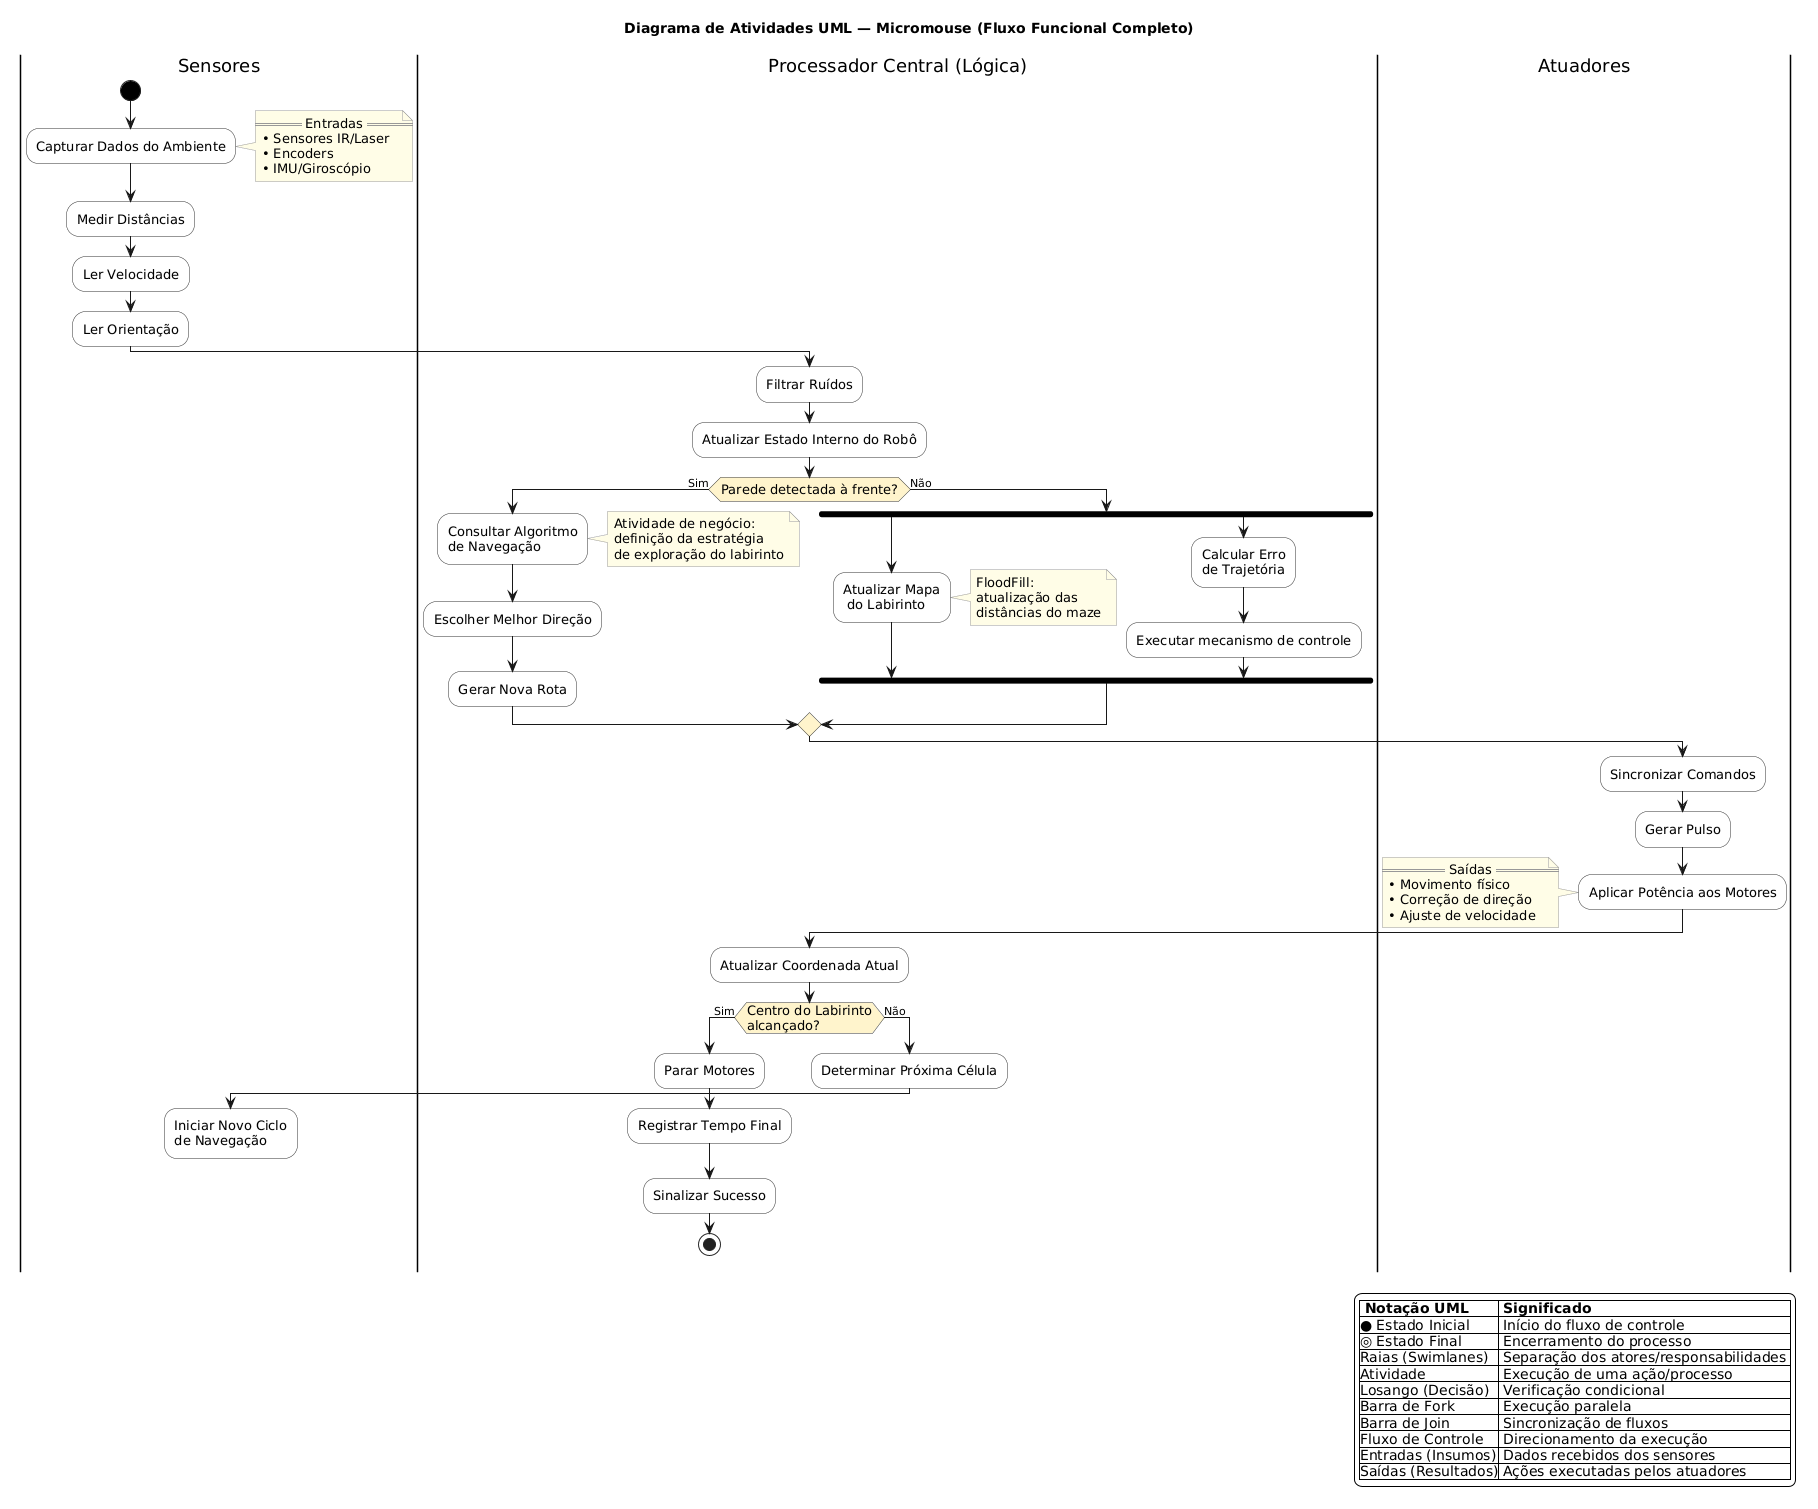
\includegraphics[width=1\linewidth]{figuras/DiagramaDeAtividadesUMLMicromouse.png}
    \caption{Diagrama de Atividades UML}
    \label{fig:placeholder}
\end{figure}



\subsection{Backlog do Produto}

O backlog do produto representa a lista priorizada de funcionalidades e requisitos que orientam o desenvolvimento do sistema Micromouse. Sua construção foi realizada a partir das Histórias de Usuário apresentadas na Tabela 5, relacionando os Requisitos Funcionais (RFs) e Não Funcionais (RNFs) definidos para o projeto.

Os Requisitos Não Funcionais foram organizados conforme a técnica URPS+ (Usabilidade, Confiabilidade, Desempenho, Suportabilidade e outros), garantindo que aspectos essenciais como estabilidade, desempenho, experiência do usuário e manutenção do sistema fossem considerados no planejamento.

Cada história de usuário inclui critérios de aceitação, requisitos associados e prioridade classificada segundo o método MoSCoW, categorizando-as em Must Have ou Should Have de acordo com sua relevância para o funcionamento autônomo do micromouse.

\begin{table}[htbp]
\begin{center}
\scriptsize
\setlength{\tabcolsep}{4pt}
\renewcommand{\arraystretch}{1.5} % Ajustado para 1.5 para melhor leitura das células com muito texto
\caption{Backlog de Histórias de Usuário para o Sistema Micromouse.}
\begin{tabular}{|c|p{5cm}|p{4cm}|p{2cm}|p{2cm}|}
\hline
\textbf{ID} & \textbf{História de Usuário} & \textbf{Critério de Aceitação} & \textbf{Requisitos} & \textbf{Propriedades} \\
\hline

\textbf{US01} & Como operador, quero visualizar os dados de consumo de bateria e velocidade média para monitorar o desempenho. & O sistema deve atualizar os dados na interface web em tempo real. & RF11, RF13 & Prioridade: Must Have \\ \hline

\textbf{US02} & Como operador, quero consultar os dados de tipo de labirinto, tempo total de execução, trajeto percorrido, status do desafio e posição do micromouse em tempo real para avaliar resultados. & Todos os dados devem ser  visíveis pós-execução. & RF03, RF15, RF17, RF18, RF19 & Prioridade: Must Have \\ \hline

\textbf{US03} & Como operador, quero que os dados das execuções sejam armazenados e permitam consulta posterior para análise histórica. & Os dados devem persistir no banco de dados e ser recuperáveis. & RF20, RF21 & Prioridade: Must Have \\ \hline

\textbf{US04} & Como operador, quero que o micromouse percorra o labirinto de forma autônoma, detectando as paredes durante a navegação e identificando a área central do mesmo.& O micromouse deve chegar a área central sem interferêcia humana, se guiando pelas paredes. & RF01, RF02, RF05 & Prioridade: Must Have 
\\ \hline

\textbf{US05} & Como operador quero que o micromouse consiga resolver labirintos de diferentes dimensões, mapeando a labirinto através da disposição das paredes e decidindo aonde ir com base nos caminhos disponíveis. & O micromouse deve usar as paredes a sua disposição e o caminho que estiver livre para percorrer o labirinto e mapear seu percurso & RF04, RF06, RF07, RF 08 & Prioridade: Must Have 
\\ \hline

\textbf{US06} & Como operador, quero que o micromouse percorra o labirinto mais rapidamente, comparado com a velocidade de mapeamento. & O micromouse deve ser mais veloz no seu percurso, depois de mapear o labirinto. & RF23 & Prioridade: Should Have \\ \hline

\textbf{US07} & Como operador, quero que conseguir visualizar e comparar os dados da trajetória percorrida, consumo de bateria, velocidade média do micromouse, tempo de execução e o mapa do labirinto por meio de uma interface web & O sistema deve exibir o consumo de bateria, velocidade média do micromouse, tempo de execução e o mapa do labirinto em tempo real na interface web. & RF09, RF10, RF12, RF14, RF16, RF22, RF24 & Prioridade: Must Have \\ \hline

\end{tabular}
\end{center}
\label{US}
\end{table}

\subsection{Descrição da Arquitetura da Solução de Software Proposta}

A arquitetura de software foi projetada para orquestrar a navegação autónoma do micromouse e fornecer uma plataforma robusta para monitorização em tempo real e armazenamento do histórico de execuções. O sistema adota o padrão \textbf{Cliente-Servidor} operando em rede local, garantindo independência de serviços externos. A aplicação web foi estruturada sob os princípios do padrão arquitetural \textbf{MVC (Model-View-Controller)}, adaptado para o desenvolvimento web moderno em componentes.

\begin{figure}
    \centering
    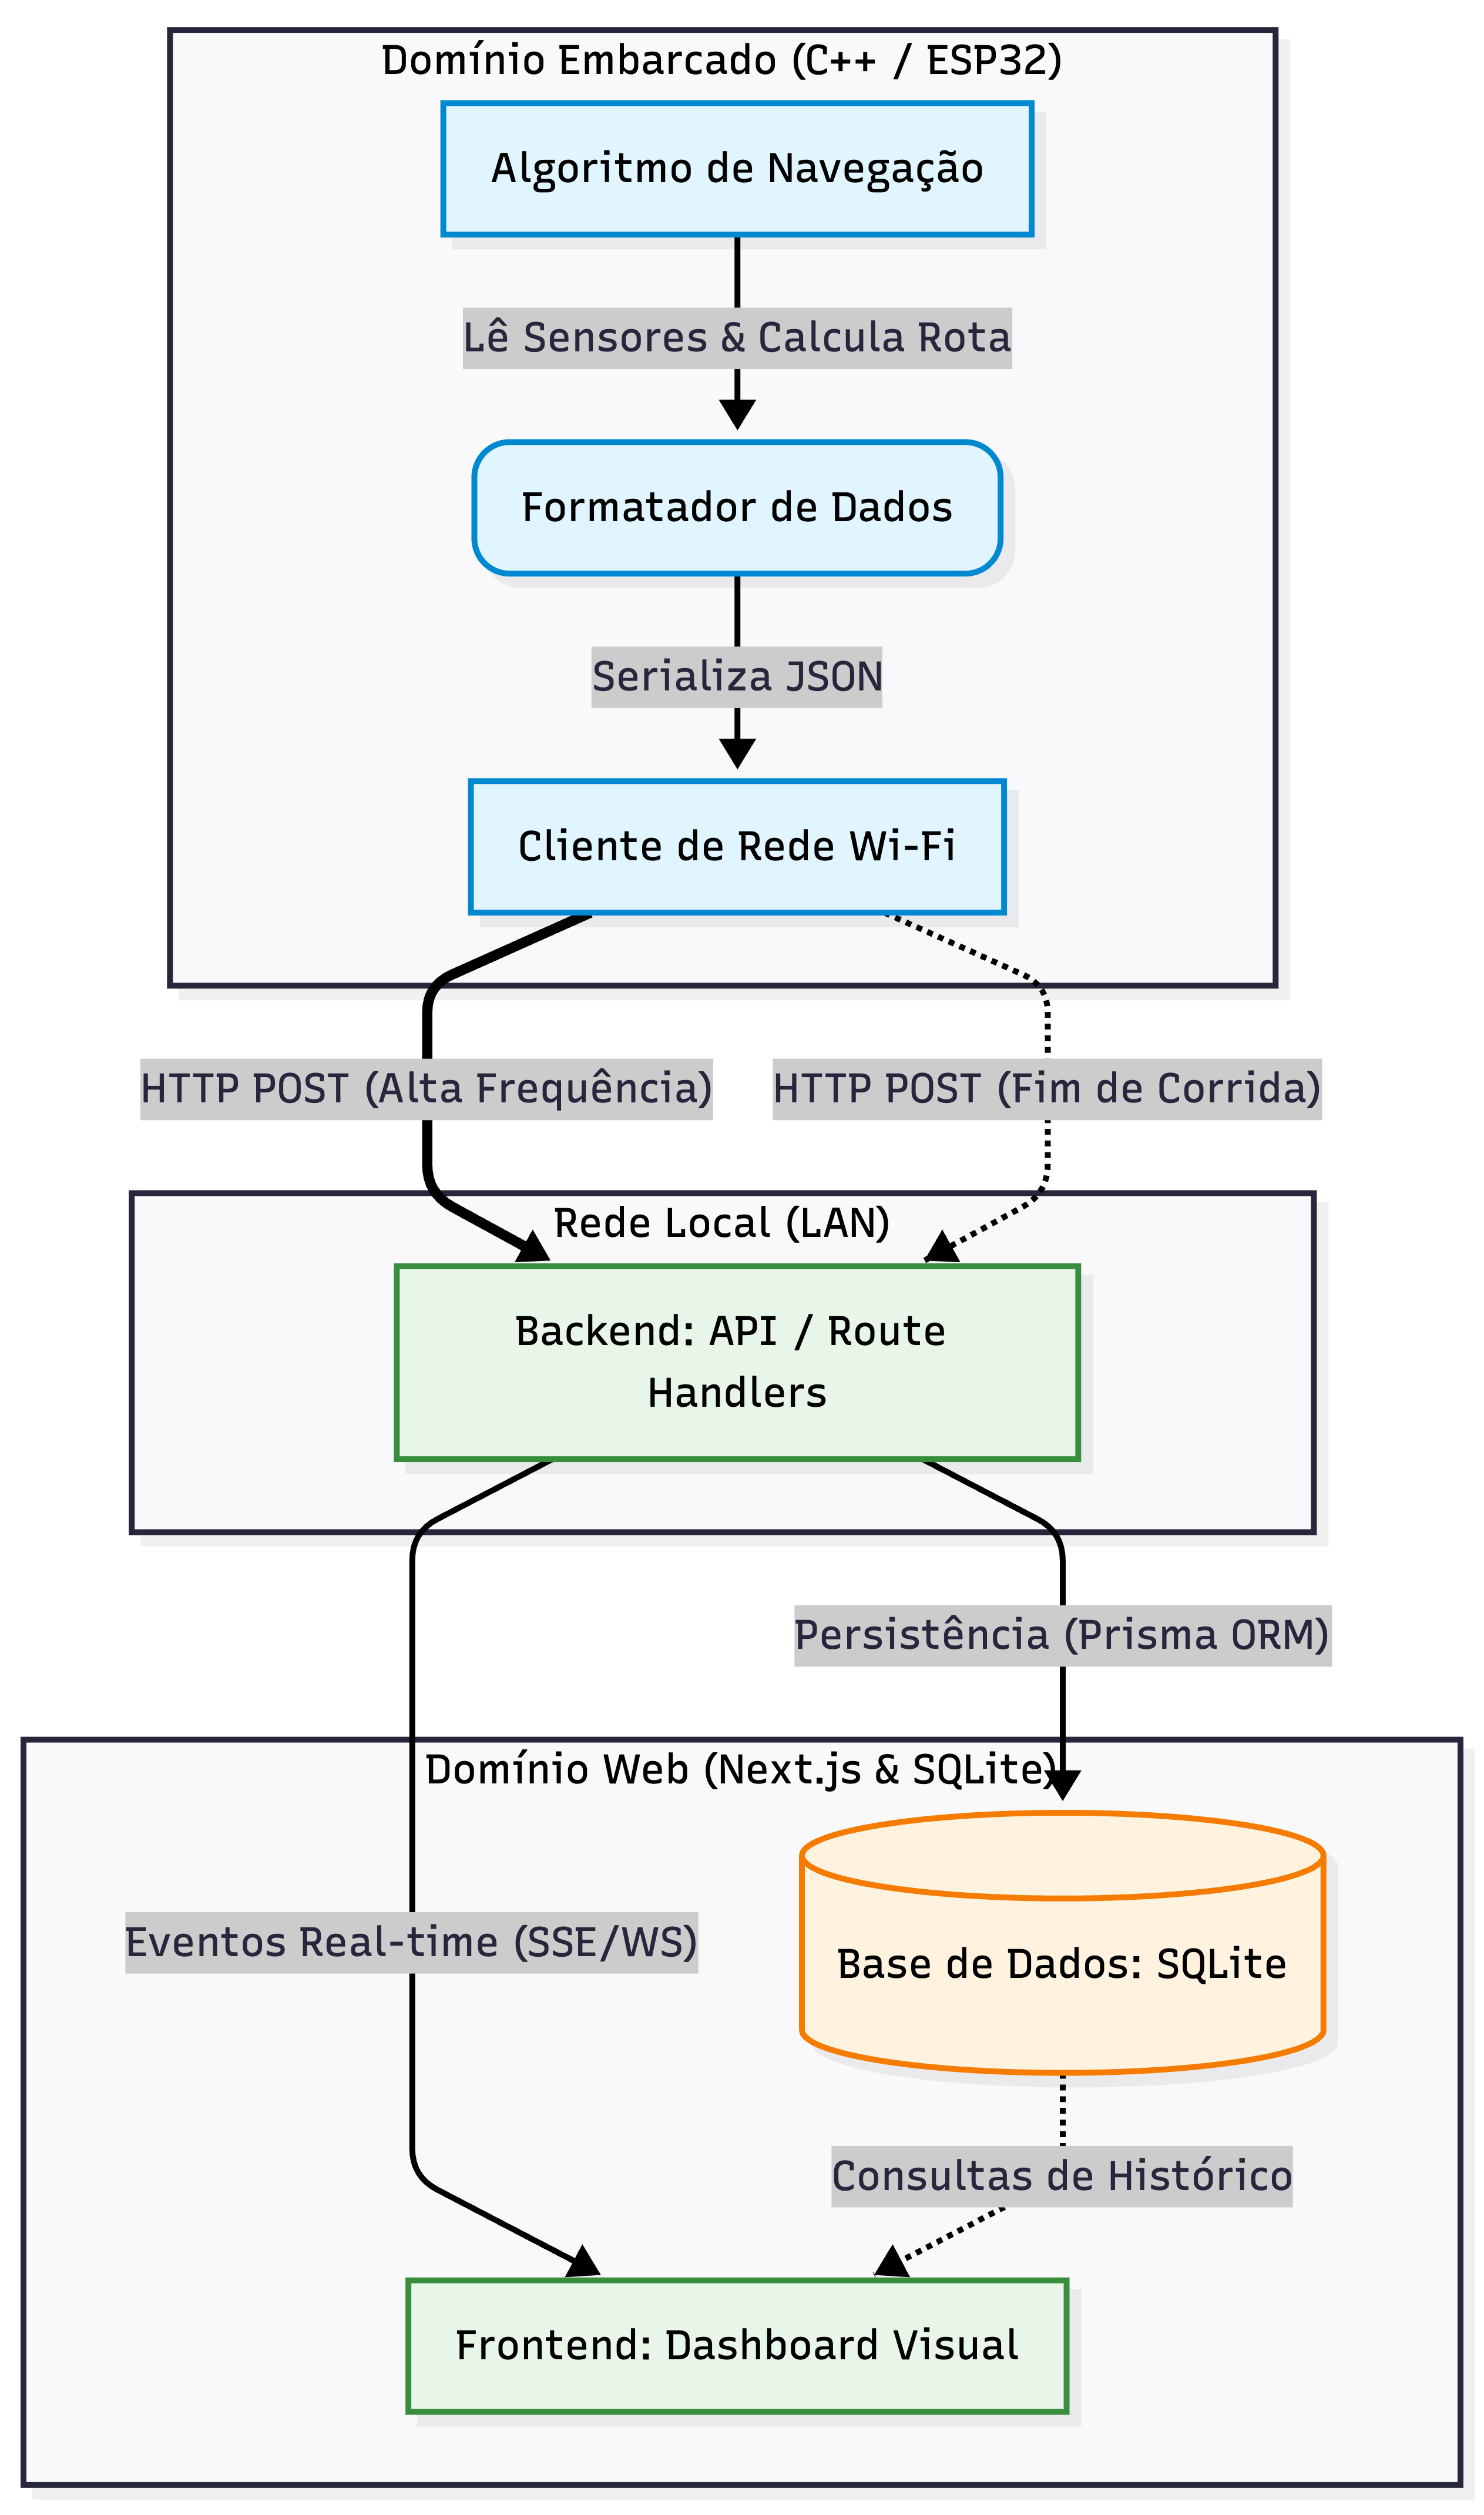
\includegraphics[width=0.5\linewidth]{figuras/diagrama_arquitetura.png}
    \caption{Diagrama da Arquitetura}
    \label{fig:placeholder}
\end{figure}

As tecnologias selecionadas para compor a solução dividem-se em dois escopos principais:
\begin{itemize}
    \item \textbf{Firmware (C++):} Linguagem escolhida pela alta performance na execução dos algoritmos de busca e mapeamento, além de permitir o controlo de baixo nível necessário para comandar atuadores e processar dados de sensores.
    \item \textbf{Sistema Web (TypeScript/JavaScript):} Utilização do framework \textbf{Next.js}, que integra API (Backend) e interface de utilizador (Frontend). Para a persistência, utiliza-se o \textbf{Prisma ORM} com base de dados \textbf{SQLite}, ideal para centralizar os dados localmente.
\end{itemize}

A arquitetura do software é detalhada a seguir, estruturada conforme as visões do modelo $4+1$ do processo unificado:

\subsubsection{Visão Lógica}
O software divide-se nos Blocos de Software Embarcado e Software Web. O \textbf{Bloco de Software Embarcado (C++)} contém a inteligência de navegação: recebe entradas do ambiente, atualiza a matriz do labirinto e toma decisões de rota. Já o \textbf{Bloco de Software Web (Next.js)} lida com todas as informações passadas pelo bloco embarcado, disponibilizando rotas de API e painéis visuais.

\subsubsection{Visão de Processos}
O código C++ opera num laço não-bloqueante para garantir a fluidez da navegação. O algoritmo processa a próxima ação e transmite os dados (mapa, velocidade, tempo e bateria) via rede local. O \textbf{Backend do Next.js} repassa os dados instantaneamente para o navegador via eventos em tempo real, enquanto o \textbf{Frontend} reage às mudanças de estado para atualizar os gráficos dinamicamente.

\subsubsection{Visão de Dados: Modelo Entidade-Relacionamento (MER)}
A camada de dados foi modelada para separar as configurações estáticas dos labirintos das métricas dinâmicas geradas pelo software. 

\begin{description}
    \item[Entidade Labirinto:] Define o ambiente virtual da prova. Atributos: \textit{id} (PK), \textit{tipo} (4x4, 8x8, 16x16), \textit{tamanho\_celula\_cm} e \textit{descricao}.
    \item[Entidade Corrida:] Regista o desempenho de cada tentativa. Atributos: \textit{id} (PK), \textit{labirinto\_id} (FK), \textit{data\_hora}, \textit{tempo\_conclusao}, \textit{velocidade\_media}, \textit{consumo\_bateria}, \textit{desafio\_cumprido} (S/N) e \textit{trajeto\_coordenadas}.
    \item[Relacionamento:] Um \textbf{Labirinto} pode possuir várias \textbf{Corridas}, mas uma \textbf{Corrida} pertence a apenas um \textbf{Labirinto} (Relação 1:N).
\end{description}

O Diagrama Entidade-Relacionamento (DER) correspondente pode ser visualizado na Figura~\ref{fig:der_micromouse}.

\begin{figure}[htbp]
    \centering
    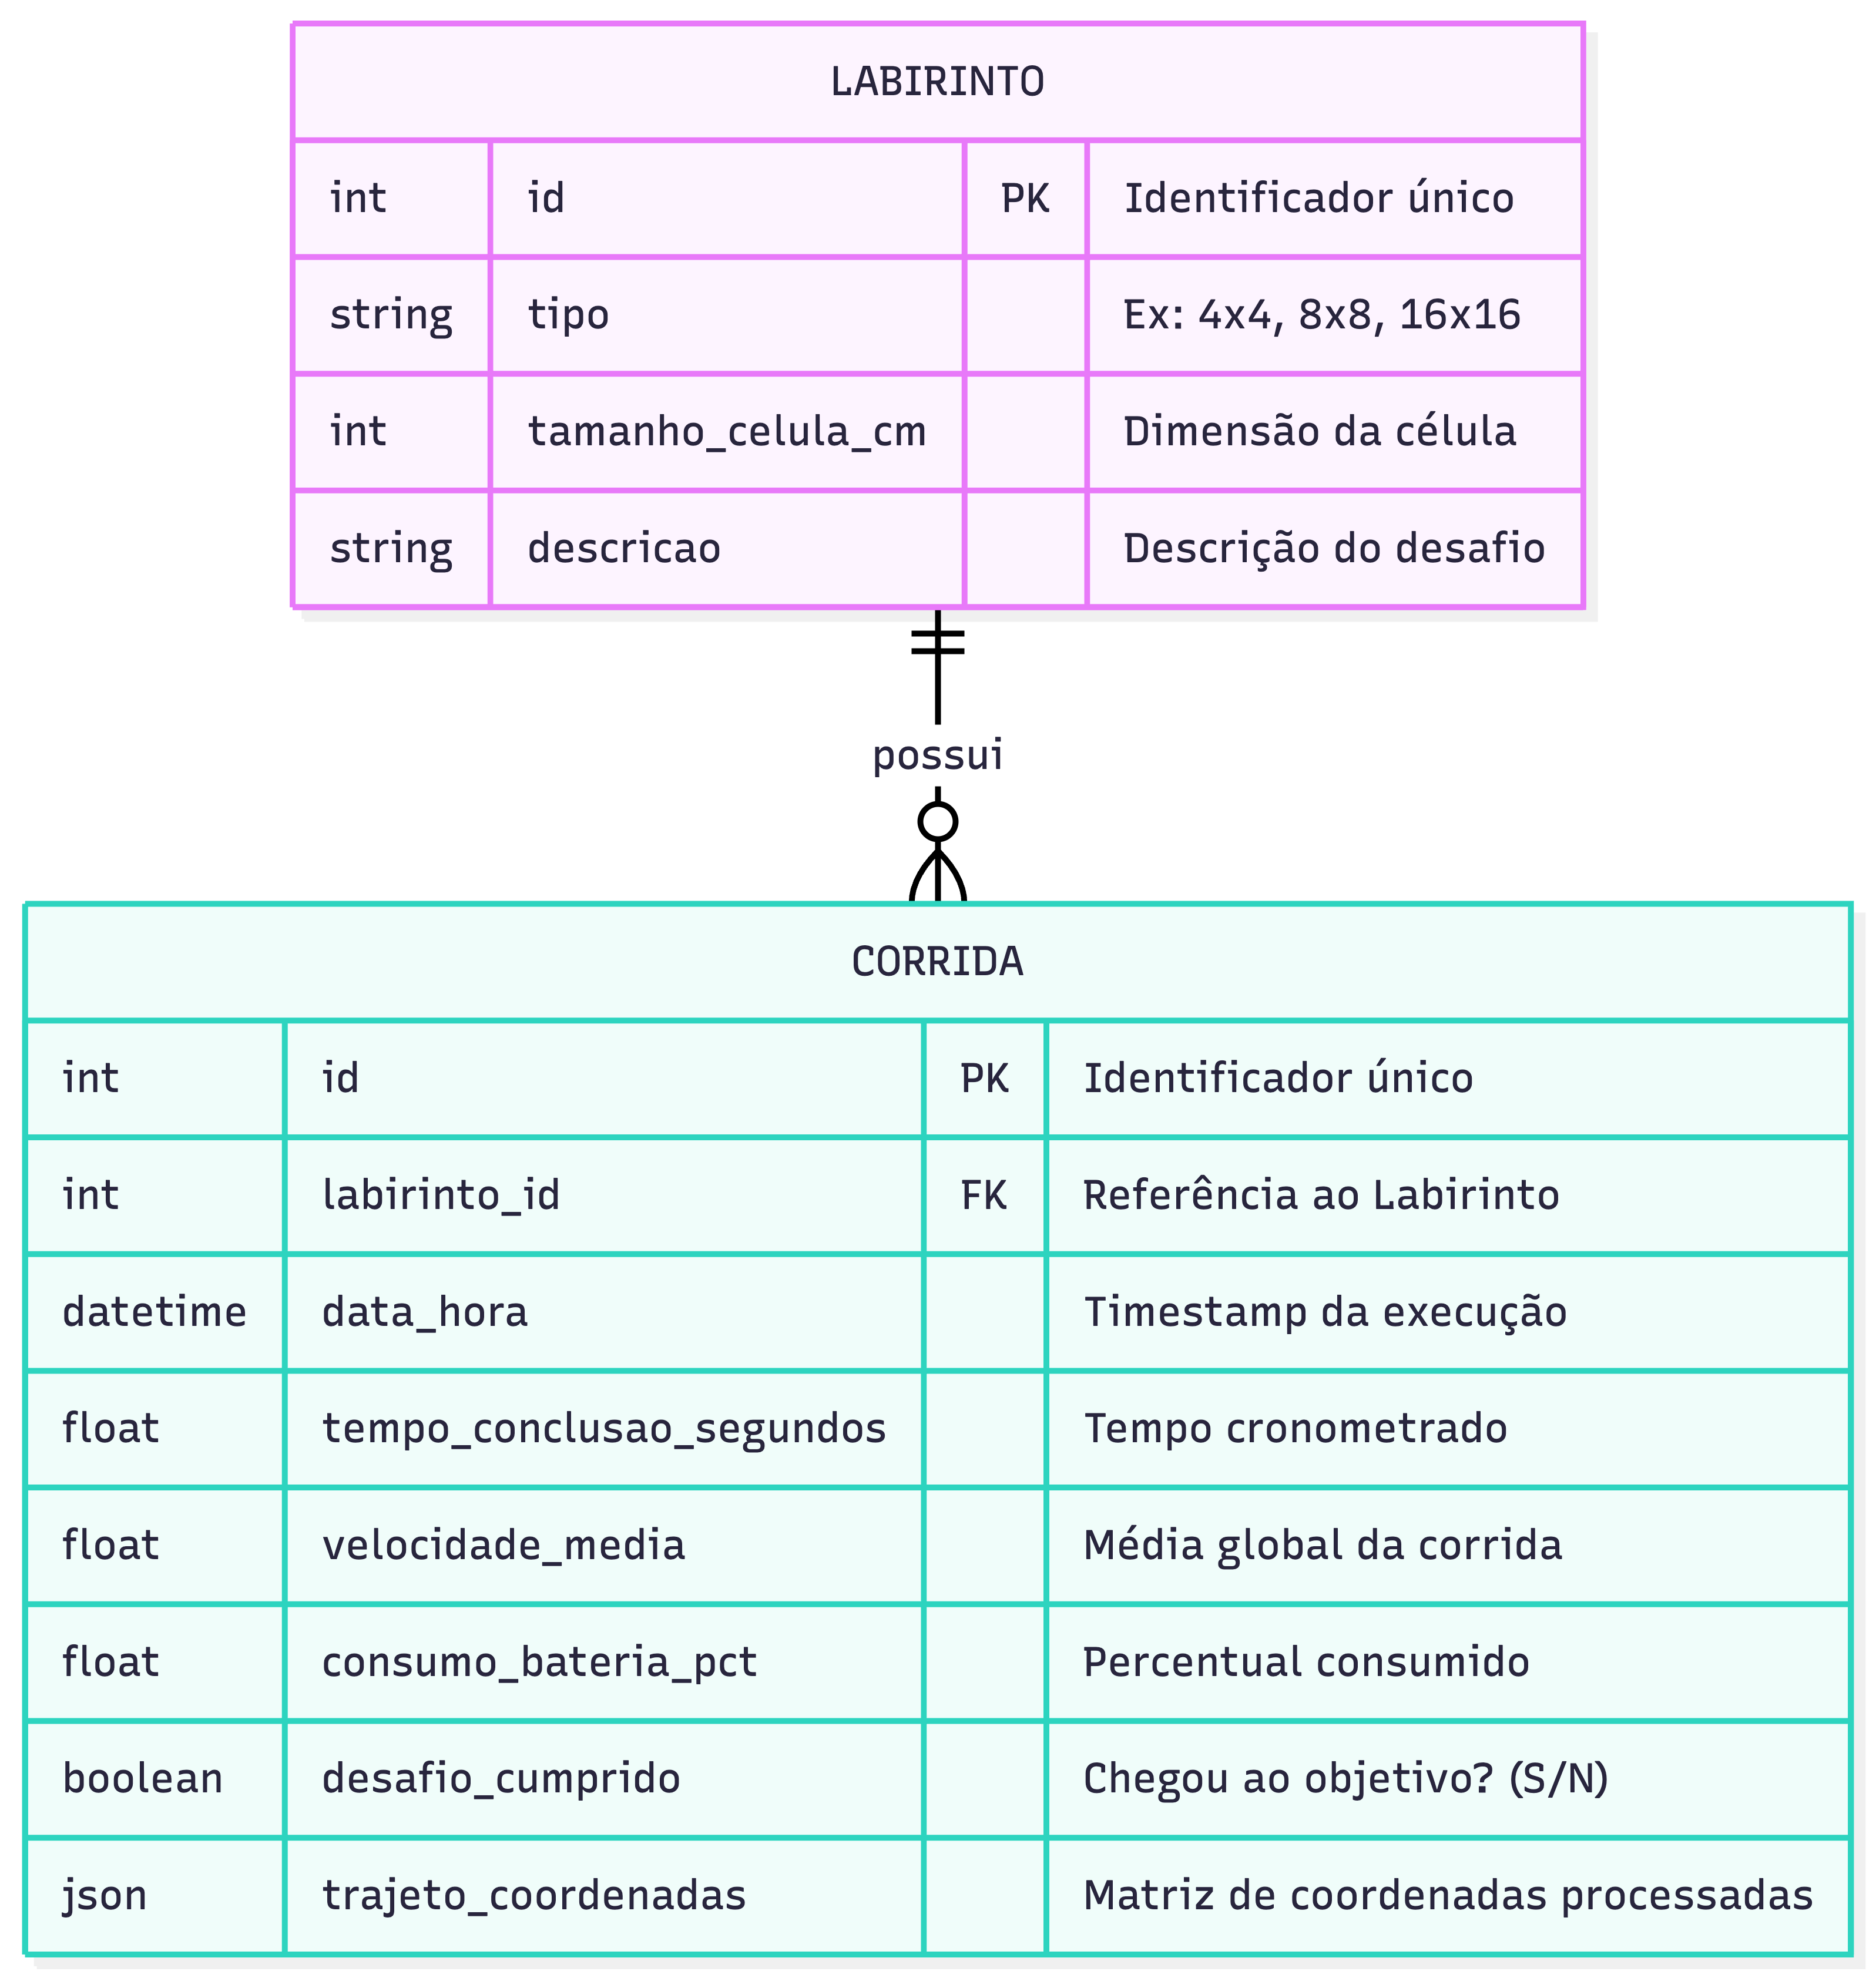
\includegraphics[width=0.5\linewidth]{figuras/diagrama_der.png}
    \caption{Diagrama Entidade-Relacionamento (DER) do Sistema.}
    \label{fig:der_micromouse}
\end{figure}

\subsubsection{Visão de Implementação e Implantação}
O código C++ é modularizado entre a lógica com o Algoritmo Frontier-Based Exploration e funções de I/O. A aplicação web segue a componentização React com comunicação tipada via Prisma. A implantação é feita em \textit{localhost} numa rede isolada para garantir latência mínima e segurança na execução.

\subsubsection{Protótipo de Alta Fidelidade no Figma}

Foi desenvolvido um protótipo de alta fidelidade no Figma para validar a interface e os fluxos de interação do sistema, incluindo a visualização do mapa de ocupação, os painéis de controle do algoritmo Frontier-Based Exploration e a retroalimentação visual em tempo real. O protótipo serviu como base para testes de usabilidade e comunicação entre a equipa de desenvolvimento e os stakeholders. O projeto está disponível no seguinte link: \href{https://www.figma.com/design/hAd6xD3YEXpLAWpT3NWGVL/Projeto-Integrado-1---Mouse?node-id=0-1&t=yfaBe6EYSQN7qefh-1}{Link do Protótipo}. E, além disso, pode ser visualizado na Figura~\ref{fig:prototipo}.

\begin{figure}[htbp]
    \centering

    \fbox{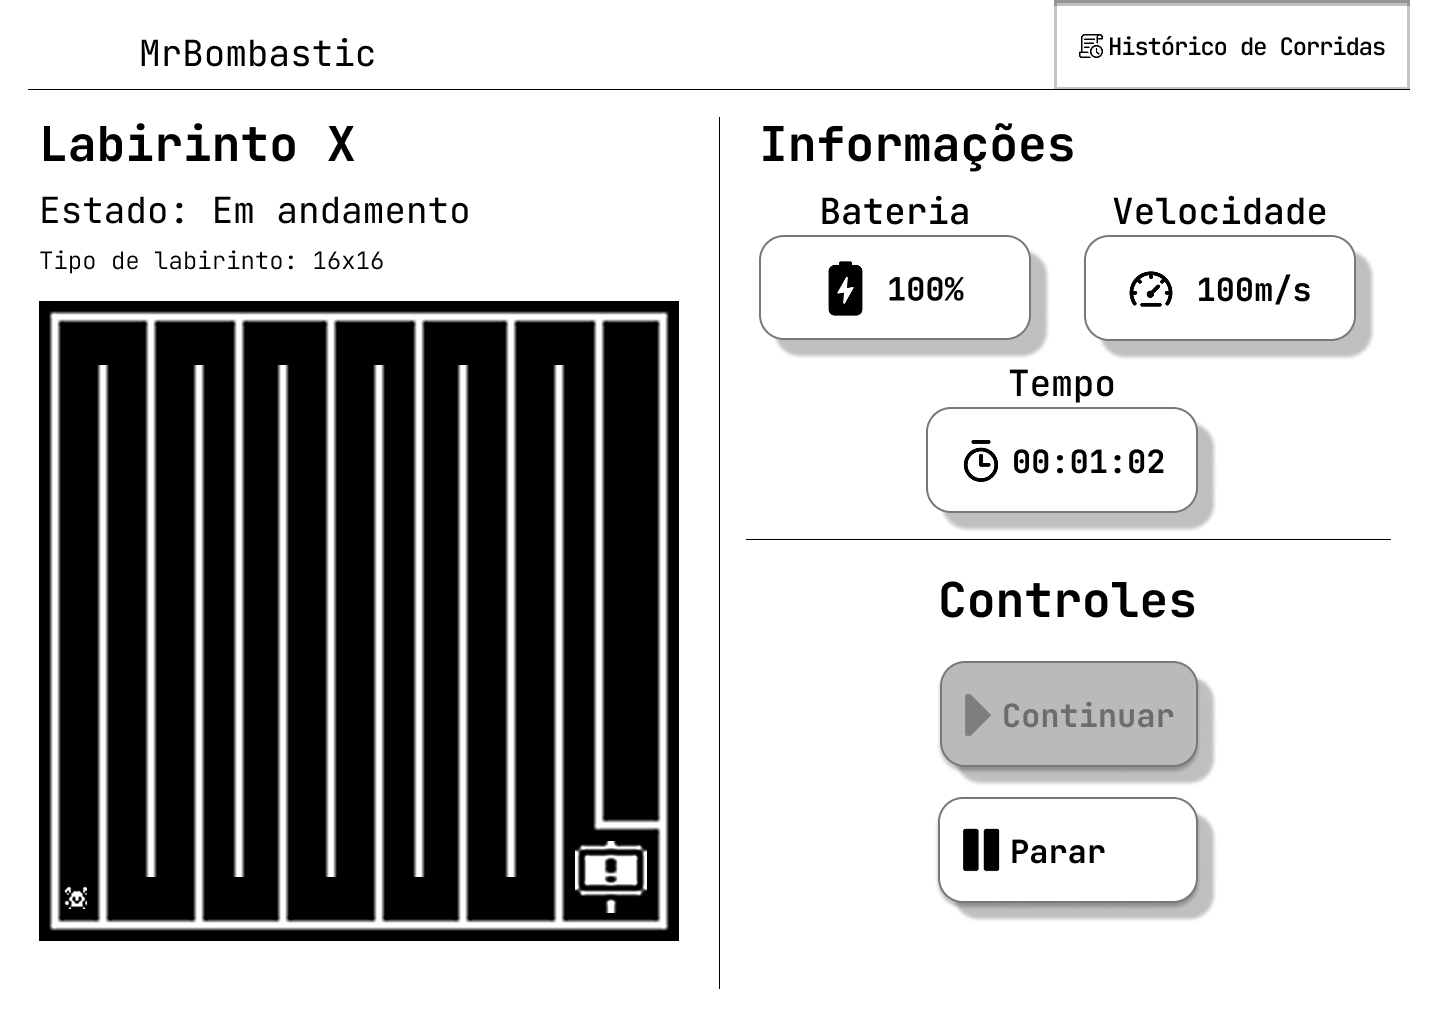
\includegraphics[width=0.4\textwidth]{figuras/tela1.png}}
    \hspace{0.5cm}
    \fbox{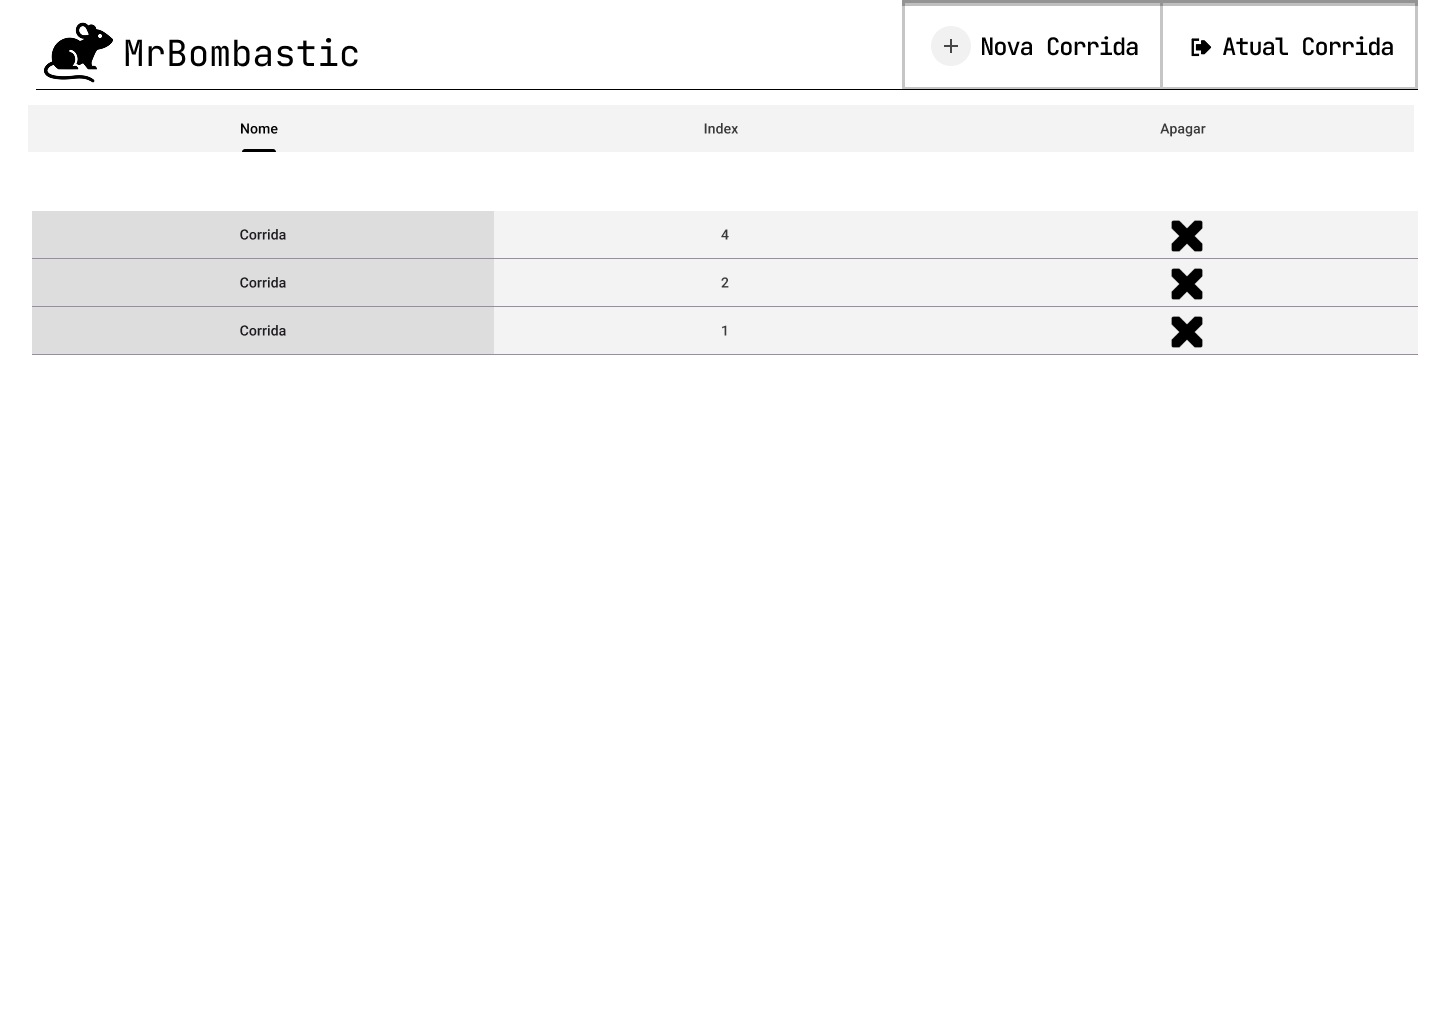
\includegraphics[width=0.4\textwidth]{figuras/tela2.png}}
     \\[0.5cm]
    \fbox{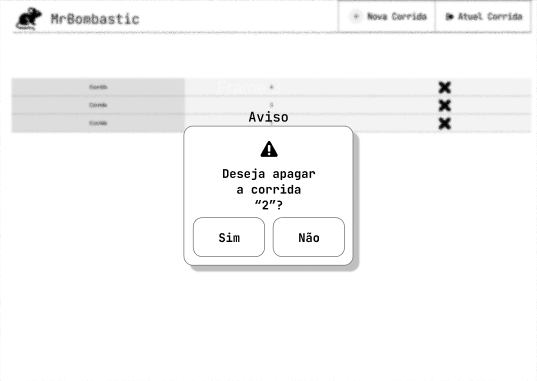
\includegraphics[width=0.4\textwidth]{figuras/tela3.png}}

    \caption{Protótipo.}
    \label{fig:prototipo}
\end{figure}

\subsection{Roteiro de Testes Funcionais}

Neste capítulo são apresentados os testes desenvolvidos para verificar o funcionamento correto do Micromouse e garantir que todos os seus módulos operem de forma confiável, precisa e segura. Para isso, foi elaborado um roteiro estruturado de testes funcionais que contempla desde a navegação básica até mecanismos de segurança, mapeamento e comunicação. A Tabela~\ref{tab:roteiro_testes} reúne cada um desses testes, descrevendo seus objetivos, condições necessárias, procedimentos adotados e resultados esperados.

\begin{table}[htbp]
    \centering
    \caption{Roteiro de testes funcionais do sistema}
    \label{tab:roteiro_testes}
    \resizebox{\textwidth}{!}{%
        \begin{tabular}{|l|p{3cm}|p{4cm}|p{3.5cm}|p{4.5cm}|p{4cm}|}
            \hline
            \textbf{Código} & 
            \textbf{Nome} & 
            \textbf{Objetivo} & 
            \textbf{Pré-condições} & 
            \textbf{Procedimentos} & 
            \textbf{Resultado Esperado} \\ 
            \hline
            
            CT-01 & 
            Início da Navegação & 
            Verificar início independente. & 
            Robô na célula inicial e ligado. & 
            1. Acionar ativação.\newline 2. Afastar as mãos e observar. & 
            Início imediato do movimento sem auxílio humano. \\ 
            \hline
            
            CT-02 & 
            Detecção de Paredes & 
            Validar sensores ToF. & 
            Robô em movimento com obstáculo à frente. & 
            1. Deixar o robô navegar.\newline 2. Observar reação frontal. & 
            Detecção da parede e mudança de trajetória antes da colisão. \\ 
            \hline
            
            CT-03 & 
            Telemetria Web & 
            Validar envio de dados Wi-Fi. & 
            Robô conectado; Interface web aberta. & 
            1. Movimentar o robô.\newline 2. Checar painel web. & 
            Exibição de velocidade e bateria com atualização em tempo real. \\ 
            \hline
            
            CT-04 & 
            Parada de Emergência & 
            Garantir parada rápida. & 
            Micromouse em movimento contínuo. & 
            1. Enviar comando de parada.\newline 2. Medir tempo de resposta. & 
            Parada total dos motores em menos de 2 segundos. \\ 
            \hline
            
            CT-05 & 
            Mapeamento & 
            Validar registro do labirinto. & 
            Labirinto estruturado e robô ativo. & 
            1. Executar ciclo de navegação.\newline 2. Conferir mapa gerado. & 
            Geração progressiva do mapa no sistema conforme exploração. \\ 
            \hline
            
            CT-06 & 
            Identificação do Objetivo & 
            Validar alcance da área central. & 
            Robô em busca da área central. & 
            1. Deixar o robô encontrar o centro.\newline 2. Observar status. & 
            Identificação correta do ponto final e sinalização de sucesso. \\ 
            \hline
        \end{tabular}%
    }
\end{table}

%\textcolor{red}{Itens fundamentais:}

%\begin{itemize}
 %   \item \textcolor{red}{ \textbf{Diagrama Atividades UML:}  descrever e explicar o fluxo do comportamento funcional do produto proposto, evidenciando, de forma clara e estruturada, como as atividades são executadas, em que ordem e sob quais condições. Esse diagrama permite compreender o funcionamento dinâmico do sistema, destacando:}

  %  \begin{itemize}
   %     \item \textcolor{red}{ os principais atores (usuários ou sistemas externos) envolvidos no processo;
    %    \item as atividades de negócio realizadas por cada ator ou pelo próprio sistema;
     %   \item os insumos (entradas) necessários para a execução das atividades;
      %  \item os resultados (saídas) gerados ao longo do fluxo;
       % \item os pontos de decisão, paralelismo e sincronização das atividades;
        %\item Entre as notações mais relevantes, destacam-se o estado iniciail e final, atividades, nós de decisão e junção, barras de bifurcação, Raias (\textit{swimlanes}) e Fluxos de controle. }
        %\end{itemize}

%    \item \textcolor{red}{\textbf{\textit{Backlog} do Produto}}
 %   \begin{itemize}
     %   \item \textcolor{red}{ Descrever os   requisitos funcionais (RF) com a técnica de documentação e especificação de história de usuário (HU);}
      %  \item \textcolor{red}{ Descrever os requisitos não-funcionais (RNF) de forma objetiva; Mais facilmente, mais rapidamente, mais responsivo, de fácil uso, são descrições subjetivas não-válidas. Um exemplo de requisito não-funcional de desempenho: ``a página deve carregar em até 5s quando em conexão 4G''. }
      %  \item \textcolor{red}{ Ao descrever os requisitos (RF e RNF), usar a  classificação MoSCoW (\textit{Must have}, \textit{Should have} e \textit{Could have}),  para auxiliar a priorização dos itens do backlog.}
       % \item \textcolor{red}{ Protótipos de interfafe gráfica do \textit{software} em alta fidelidade.}
      %  \begin{itemize}
         %   \item \textcolor{red}{\textbf{ Todas HUs devem conter sua descrição (Eu-Como-Para), critérios de aceitação e protótipos de interface, documentadas no github. }}
         %   \end{itemize} 

    %    \end{itemize}

   % \item \textcolor{red}{ \textbf{Descrição da arquitetura da solução de \textit{software} proposta:}}
   % \begin{itemize}
    
       % \item \textcolor{red}{ Esta subseção deve contemplar o documento de arquitetura do sistema e deve ser estruturado segundo as visões (4+1) previstas no processo unificado (UP): lógica, de processos;  implementação, implantação e dados (substuirá a visão de casos de uso).}
        
        %\item \textcolor{red}{ Propósito do \textit{software} (qual o seu papel no sistema);}
      %  \item \textcolor{red}{ Padrão adotado: MVC, MVP, Microsserviços, Monolítico, etc (Justificar);}
      %  \item \textcolor{red}{ Linguagens de programação: Java, Python, C\#, JavaScript, etc.}
       % \item \textcolor{red}{ \textit{Frameworks} e bibliotecas: Spring Boot, .NET Core, React, Angular, Django, etc.}
       %     \item \textcolor{red}{ Banco de dados: Relacional (PostgreSQL, MySQL, etc) X NãoSQL (MongoDB,etc). }
       % \item \textcolor{red}{Persistência de dados: Modelo Entidade‑Relacionamento (MER) e seu respectivo Diagrama Entidade‑Relacionamento (DER), aplicáveis quando a solução utiliza banco de dados relacional; alternativamente, diagrama de estrutura de documentos, empregado nos casos em que a arquitetura adota banco de dados não relacional.}
       %  \end{itemize}     
    
   % \item \textcolor{red}{\textbf{ Roteiro de testes funcionais:} }
   % \begin{itemize}
       % \item \textcolor{red}{Código do caso de teste;}
      %  \item \textcolor{red}{Nome do caso de teste;}
     %   \item \textcolor{red}{ Objetivo do caso de teste;}
   %     \item \textcolor{red}{ Pré-condições do sistema para o teste ser realizado, quando se aplicar;}
    %    \item \textcolor{red}{ Descrição dos procedimentos a serem executados para o teste;}
     %   \item \textcolor{red}{ Resultado esperado para o teste ser aprovado (pós-condição após realizado o teste);}
  %  \end{itemize}
%\end{itemize}


% \textcolor{red}{Com relação ao \textit{software}, será necessário apresentar os seguintes itens: % pacotes de componentes de \textit{software}, suas funções e características, e explicar as decisões de projeto:
% \begin{enumerate}
%     \item Um diagrama do processo de negócio do problema que a máquina se propõe a resolver (BPNM) – não é UML, mas é fundamental para entender como o sistema se comporta como um todo, incluindo o usuário;
%     \item Lista de casos de uso (backlog do sistema). Backlog funcional;
%     \item Lista de requisitos não-funcionais a serem satisfeitos pelo sistema;
%     \item Diagrama de casos de uso: mostrando os requisitos funcionais, seus atores e como eles interagem entre si;
%     \item Diagrama de Classes: apresentando quais dados são manipulados pelo sistema (internamente e externamente – ex.: resultados de experimentos);
%     \item Diagrama de arquitetura, identificando todos os componentes da máquina e suas iterações com o software;
%     \item Diagrama de estados da máquina (sistema);
%     \item Descrição dos testes dos componentes da máquina e dos testes funcionais que deveriam ser feitos para avaliar o funcionamento da máquina e identificar defeitos. São importantes os testes unitários (componentes) e de integração (conjunto de componentes) e o roteiro de testes.
% \end{enumerate}
% }
%\textcolor{red}{Com relação ao \textit{software}, será necessário apresentar pacotes de componentes de \textit{software}, suas funções e características, e explicar as decisões de projeto.}